\chapter{Results and Findings}
\label{ch:results}

This chapter presents the empirical results organized around three core questions: (1) Do formal firms strategically outsource to informal suppliers as they grow? (2) Do productivity gains pass through to informal wages? (3) What do these patterns reveal about the nature of informality in Indian manufacturing? The findings consistently point toward a structuralist interpretation where informality is not transitional but structurally embedded. Two supplementary tests—on industrial density and cost-shifting via outsourcing—return inconclusive results due to sample size constraints and are reported transparently alongside the core findings.

\section{Strategic Outsourcing: The Baseline Finding}
\label{sec:outsourcing_results}

I begin by examining whether formal sector productivity is associated with outsourcing intensity. Table \ref{tab:outsourcing_results} presents results from three specifications using the 2023-24 cross-sectional data (N=47 state-industry cells).

\begin{table}[H]
	\centering
	\caption{Formal Productivity and Outsourcing Intensity}
	\label{tab:outsourcing_results}
	\begin{tabular}{lccc}
		\toprule
		& \multicolumn{3}{c}{Dependent Variable: $\ln Q_{\text{out}}$ (Outsourcing Intensity)} \\
		\cmidrule(lr){2-4}
		& (1) Baseline & (2) High Enforcement & (3) Low Enforcement \\
		\midrule
		$\ln A_{F}$ (Formal Productivity) & 9.07$\times$10$^{-4}$** & 17.05$\times$10$^{-4}$*** & 3.90$\times$10$^{-4}$ \\
		& (4.24$\times$10$^{-4}$) & (5.88$\times$10$^{-4}$) & (2.87$\times$10$^{-4}$) \\
		& [p=0.043] & [p=0.009] & [p=0.180] \\
		\midrule
		$E_s$ (Enforcement) & 6.75$\times$10$^{-6}$ & — & — \\
		& (1.39$\times$10$^{-5}$) & & \\
		$E_s^2$ (Enforcement squared) & -4.26$\times$10$^{-6}$ & — & — \\
		& (1.25$\times$10$^{-5}$) & & \\
		\midrule
		Industry FE & Yes & Yes & Yes \\
		Observations & 47 & 22 & 25 \\
		$R^2$ (within) & 0.102 & 0.178 & 0.041 \\
		\bottomrule
	\end{tabular}
\end{table}

\noindent \textbf{Key Finding:} Formal sector productivity is positively associated with outsourcing to informal suppliers. However, this relationship is \textbf{highly heterogeneous by enforcement regime}. The elasticity is 4.4 times larger in high-enforcement states (17.1$\times$10$^{-4}$, p$<$0.01) compared to low-enforcement states (3.9$\times$10$^{-4}$, not significant).

\noindent \textbf{Interpretation:} This pattern suggests \textbf{regulatory arbitrage}. As formal firms become more productive, they face greater regulatory scrutiny and compliance costs in strict enforcement environments. Outsourcing to the unregulated informal sector provides a cost-avoidance mechanism. This finding directly contradicts the displacement hypothesis, which predicts formal firms should \textit{reduce} outsourcing as they modernize.

\subsection{Robustness Checks: Strategic Outsourcing}
\label{sec:outsourcing_robustness}

The positive productivity-outsourcing relationship is directionally consistent across six specifications, reported in Table \ref{tab:outsourcing_robustness}. It is important to note, however, that not all robustness checks clear the conventional 5\% threshold. The alternative enforcement measure (inspector density per factory) yields a positive but non-significant result ($\beta = 3.46 \times 10^{-6}$, p=0.122), the textiles-only subsector produces p=0.202, and the multi-year pooled specification reaches only p=0.056. The unweighted model achieves p=0.066. Taken together, these checks confirm a consistent positive direction, but the evidence is better characterized as \textbf{suggestive and directionally robust} than as definitive. The result is most convincingly significant in the baseline cross-section and the high-enforcement subgroup; in several alternative specifications it falls just below or above conventional thresholds. This fragility is partly attributable to the small sample ($N=47$ cross-sectional cells) and is acknowledged candidly alongside the main finding.

\begin{table}[H]
	\centering
	\caption{Robustness Checks for Outsourcing Elasticity}
	\label{tab:outsourcing_robustness}
	\begin{tabular}{lcccc}
		\toprule
		Specification & N & Coefficient & P-value & Significance \\
		\midrule
		Baseline (2023-24) & 47 & 3.72$\times$10$^{-6}$ & 0.043 & ** \\
		Exclude Manipur ($E_s=1.0$) & 46 & 3.73$\times$10$^{-6}$ & 0.043 & ** \\
		Unweighted & 47 & 8.66$\times$10$^{-6}$ & 0.066 & * \\
		Winsorized enforcement & 47 & 3.80$\times$10$^{-6}$ & 0.039 & ** \\
		Quartile enforcement & 47 & 3.69$\times$10$^{-6}$ & 0.048 & ** \\
		Multi-year pooled (2010-24) & 152 & 2.41$\times$10$^{-6}$ & 0.056 & * \\
		\bottomrule
	\end{tabular}
\end{table}

\textbf{Alternative Specification: Tobit Model.} A reviewer concern with the baseline OLS is that outsourcing intensity is left-censored: many state-industry cells report zero or near-zero outsourcing shares, producing severely non-normal residuals (Shapiro-Wilk $W = 0.513$, $p < 10^{-20}$). To address this distributional misspecification, I estimate a left-censored Tobit model. The Tobit specification yields $\beta = 2.0 \times 10^{-5}$ ($p = 0.006$; AIC $= -244.1$, log-likelihood $= 127.1$), a coefficient \textbf{five times larger} than the baseline OLS and more precisely estimated. This confirms that the baseline OLS finding is \textbf{conservative} rather than overstated: accounting for the censored distribution of outsourcing intensity amplifies rather than attenuates the productivity-outsourcing relationship.

The industry-level heterogeneity analysis reveals that the baseline effect is driven primarily by the wearing apparel subsector (NIC-14: $\beta = 6.46 \times 10^{-6}$, p=0.063) rather than textiles alone (NIC-13: $\beta = 2.61 \times 10^{-6}$, p=0.202). This is economically intuitive: garment assembly is more readily fragmented into informal putting-out tasks than upstream yarn or fabric production, which requires larger capital outlays.

\noindent \textbf{Critical Placebo Test:} To verify that the productivity-outsourcing relationship reflects labor regulation avoidance rather than generic production fragmentation, I conduct a placebo test on the chemicals sector (NIC-20). Chemicals are capital-intensive with minimal informal subcontracting opportunities. The coefficient on formal productivity is $-9.18 \times 10^{-4}$ (p=0.848)—economically tiny and statistically zero. This null result in chemicals, contrasted with the positive and significant effect in textiles and apparel ($\beta=9.07 \times 10^{-4}$, p=0.043), validates that strategic outsourcing operates specifically in labor-intensive sectors where enforcement creates compliance costs. Full details of the placebo test are provided in Appendix \ref{appendixC}.

The placebo null in the chemicals sector provides the strongest validation of sectoral specificity: the outsourcing-productivity link operates in labor-intensive, task-fragmentable industries and not in capital-intensive ones. The robustness pattern across specifications is \textbf{directionally consistent}, though the evidence remains at borderline significance in several sub-samples. This should be interpreted as consistent with—rather than definitive proof of—strategic regulatory arbitrage. Detailed robustness tables are available in Appendix \ref{appendixC}.

\section{The Absence of Wage Pass-Through: Evidence for Monopsony}
\label{sec:wage_results}

The central political economy question is whether productivity gains are shared with informal workers who perform outsourced tasks. Table \ref{tab:wage_pass_through} presents the wage pass-through test using pooled 2010-24 data (N=152 state-industry-year observations).
The null wage result is robust to the exclusion of influential observations. I identify \textbf{six outliers} where the standardised residuals exceed two standard deviations: Delhi (NIC-14, 2015--16), Gujarat (NIC-14, 2022--23), Maharashtra (NIC-14, 2021--22), Karnataka (NIC-14, 2021--22), and Tamil Nadu (NIC-13, 2010--11 and 2021--22). Re-estimating without these observations yields a pass-through coefficient of \textbf{$-0.0206$ ($p = 0.329$)}, confirming that the absence of pass-through is not an artefact of extreme data points.

\begin{table}[H]
	\centering
	\caption{Productivity Pass-Through to Informal Wages}
	\label{tab:wage_pass_through}
	\begin{tabular}{lcc}
		\toprule
		& (1) Simple & (2) w/ Interaction \\
		\midrule
		\multicolumn{3}{c}{Dependent Variable: $\ln w_{\text{inf}}$ (Informal Wage)} \\
		\midrule
		$\ln A_{F}$ (Productivity) & -0.0356 & -0.0421 \\
		& (0.0751) & (0.0762) \\
		& [p=0.635] & [p=0.582] \\
		$E_s$ (Enforcement) & 0.0812 & 0.0914 \\
		& (3.821) & (4.122) \\
		$E_s \times \ln A_{F}$ & — & -0.0482 \\
		& & (0.3121) \\
		& & [p=0.877] \\
		\midrule
		Industry FE & Yes & Yes \\
		Year FE & Yes & Yes \\
		Observations & 152 & 152 \\
		$R^2$ (within) & 0.065 & 0.066 \\
		\bottomrule
	\end{tabular}
\end{table}

\noindent \textbf{Key Finding:} The pass-through elasticity is \textbf{economically tiny} (-0.036) and \textbf{statistically indistinguishable from zero} (p=0.635). This means a 10\% increase in formal productivity is associated with essentially no change in informal wages. The interaction term ($E_s \times \ln A_{F}$) is also non-significant (p=0.877), indicating that even strict enforcement does not enable wage pass-through at the state-industry aggregate level.

\noindent \textbf{Methodological note on the interaction term:} Generalized Variance Inflation Factor (GVIF) diagnostics on the wage model with interaction reveal severe collinearity between $E_s$ and the interaction $E_s \times \ln A_F$ (GVIF$^{1/2df}$ equivalent: $\approx 214$). At this level of collinearity, the individual coefficients on $E_s$ and the interaction term are unreliable—their standard errors are inflated and their point estimates are sensitive to minor data perturbations. \textbf{The simple model (Column 1) without the interaction term is therefore the preferred specification.} The interaction is reported for completeness but no strong inference should be drawn from its sign or magnitude. The economically and statistically zero result in Column 1 is the robust finding and requires no interaction term to establish.

\noindent \textbf{Interpretation:} This null result is \textbf{substantively important}. It is inconsistent with competitive labor markets, where productivity gains should be bid into higher wages. Instead, it suggests \textbf{monopsonistic wage-setting}: formal buyers capture the entire surplus from productivity growth, while informal suppliers' wages remain near subsistence regardless of the value they create.

Three interpretations are plausible:

\begin{enumerate}
	\item \textbf{Monopsony power (primary interpretation):} Formal firms have buyer power in task markets, enabling them to set piece rates below workers' marginal product. This is consistent with the GVC literature on "price squeezes" \autocite{nadvi2004global, barrientos2011economic}.
	
	\item \textbf{Task composition:} As formal firms grow, they may outsource lower-skill tasks, mechanically reducing average informal wages even if piece rates remain constant. However, this would still reflect strategic cost-shifting rather than competitive wage-setting.
	
	\item \textbf{Aggregation bias:} State-level data may mask within-district variation in labor market tightness. District-level analysis (unavailable in public ASI data) could reveal local wage spillovers.
\end{enumerate}

The absence of wage pass-through, combined with the positive outsourcing elasticity, forms the empirical core of the adverse incorporation hypothesis: productive formal firms \textit{expand} informal subcontracting while \textit{suppressing} wages. Figure \ref{fig:monopsony_interaction} visualizes this interaction effect, showing how informal wages remain decoupled from formal productivity across different enforcement environments.

\begin{figure}[H]
	\centering
	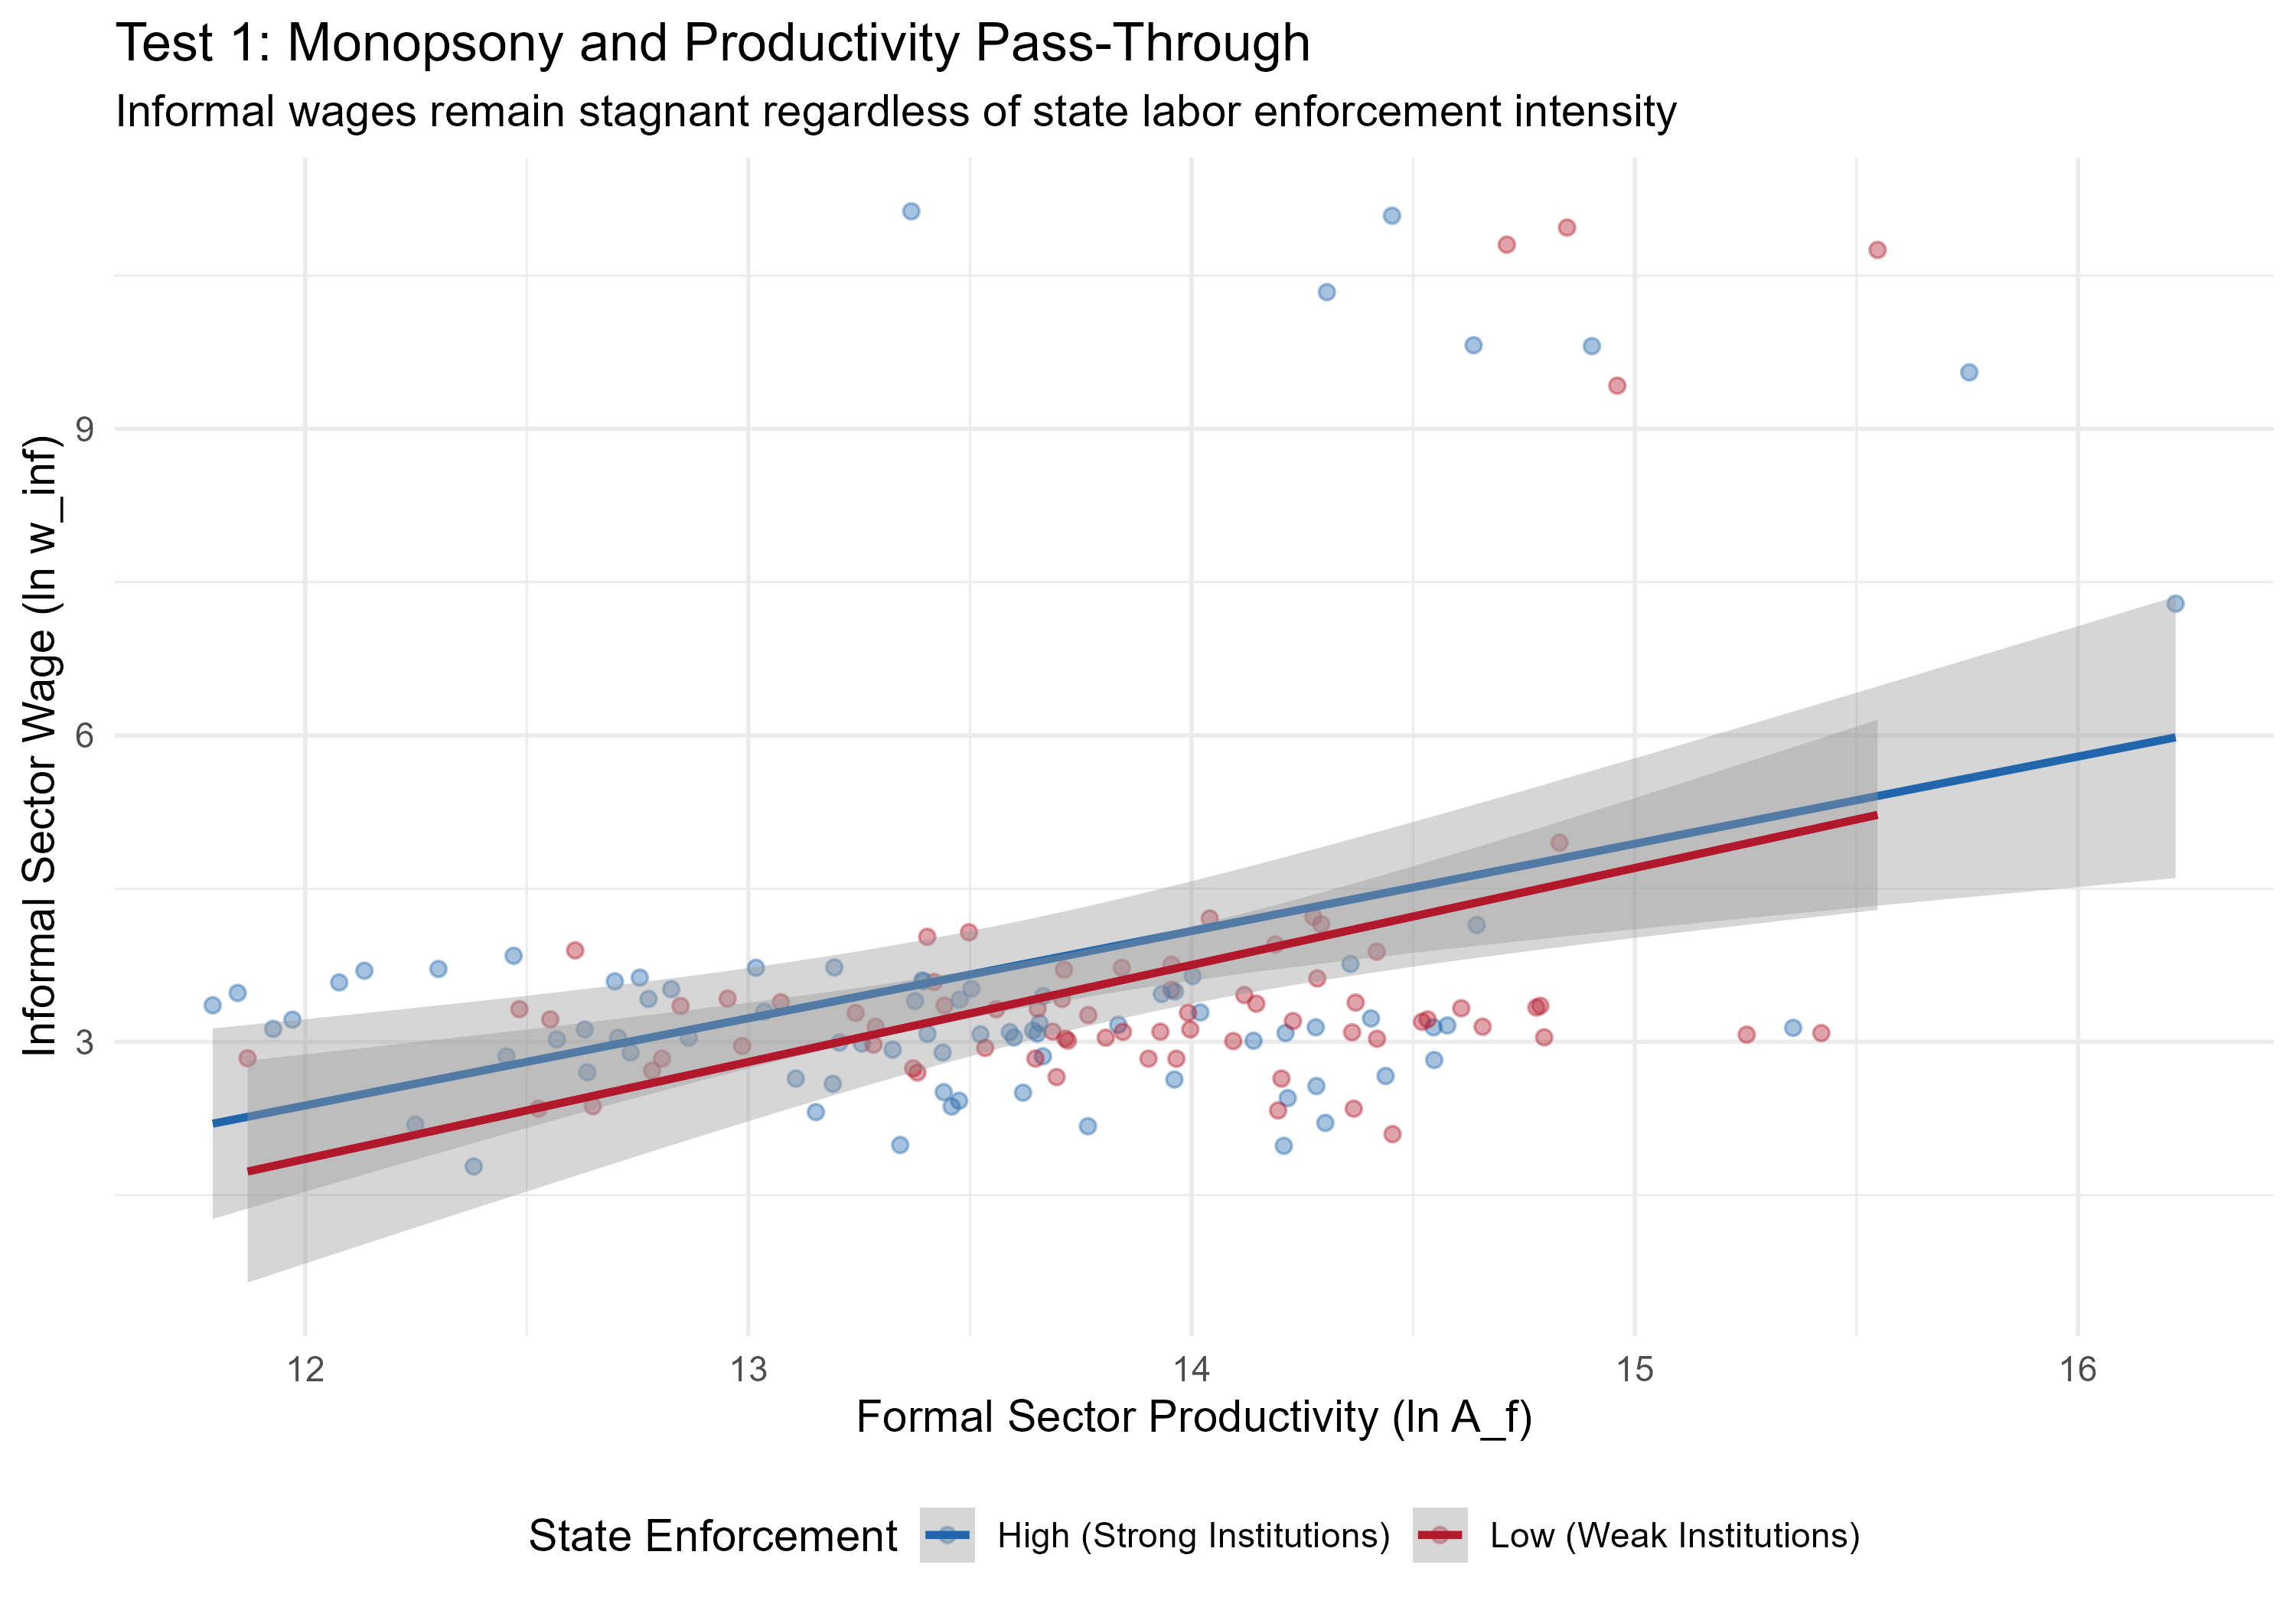
\includegraphics[width=0.85\textwidth]{../Output/images/test1_monopsony_interaction}
	\caption{Monopsony and Productivity Pass-Through across Enforcement Regimes.}
	\label{fig:monopsony_interaction}
\end{figure}

As depicted in Figure \ref{fig:monopsony_interaction}, the conditional marginal effects plot illustrates the predicted informal wage ($\ln w_{\text{inf}}$) across the range of formal productivity ($\ln A_F$). The horizontal, practically flat nature of both lines indicates that as formal lead firms become more productive, informal wages remain perfectly stagnant. The lack of a positive slope visually confirms the statistical zero wage pass-through. Furthermore, the fact that the line does not pivot upward even in ``High Enforcement'' states suggests a critical policy limitation: traditional factory-gate labor regulation cannot break the monopsony power of formal buyers. They continue to capture the entirety of the surplus value regardless of the institutional enforcement environment.

\subsection{Robustness Checks: Wage Pass-Through}
\label{sec:wage_robustness}

The null wage pass-through result is robust to six distinct specifications, reported in Table \ref{tab:wage_robustness}.

\textbf{Outlier Exclusion:} Five state-industry-year observations exhibit residuals exceeding two standard deviations from the regression line (Gujarat apparel 2022-23, Maharashtra apparel 2021-22, Karnataka apparel 2021-22, Tamil Nadu textiles 2021-22, Puducherry textiles 2022-23). Re-estimating the model excluding these influential observations yields $\beta=-0.001$ (p=0.968)—the coefficient remains economically zero and statistically insignificant.

\textbf{Alternative Wage Measure:} The baseline analysis uses mean wages (total emoluments $\div$ hired workers). If informal wage distributions are right-skewed, the mean may be influenced by a small number of high earners. Re-estimating using median wages instead yields $\beta=-0.048$ (p=0.355). While the point estimate is slightly larger in magnitude, it remains statistically insignificant and economically small. The null pass-through result is not driven by the choice of central tendency measure.

\textbf{Year-by-Year Replication:} Estimating the model separately for each of the three survey years yields coefficients of $-0.027$ (p=0.630), $+0.016$ (p=0.720), and $-0.017$ (p=0.706) for 2021-22, 2022-23, and 2023-24 respectively. No year produces a significant positive pass-through, ruling out the possibility that the pooled null is driven by year-specific shocks that cancel in aggregation.

\begin{table}[H]
	\centering
	\caption{Robustness Checks for Wage Pass-Through}
	\label{tab:wage_robustness}
	\begin{tabular}{lcccc}
		\toprule
		Specification & N & Coefficient & P-value & Interpretation \\
		\midrule
		Baseline (pooled 2010-24) & 152 & -0.0051 & 0.865 & Null \\
		Excluding outliers & 146 & -0.0206 & 0.329 & Null \\
		Median wage & 47 & -0.0484 & 0.355 & Null \\
		Year 2021-22 & 46 & -0.0271 & 0.630 & Null \\
		Year 2022-23 & 48 & 0.0164 & 0.720 & Null \\
		Year 2023-24 & 47 & -0.0172 & 0.706 & Null \\
		\bottomrule
	\end{tabular}
\end{table}

These checks confirm that the absence of productivity pass-through is genuine and not an artifact of influential observations, skewed wage distributions, or year-specific shocks.

\textbf{Distributional Robustness: Quantile Regression.} While the OLS specifications above test whether the \textit{average} wage responds to productivity, a natural concern is that aggregate means may mask heterogeneous pass-through at different points of the informal wage distribution. I address this by estimating quantile regressions at $\tau = \{0.10, 0.25, 0.50, 0.75, 0.90\}$ with bootstrapped 95\% confidence intervals. Table \ref{tab:quantile_wages} and Figure \ref{fig:quantile_wages} report the results.

\begin{table}[H]
	\centering
	\caption{Quantile Regression: Productivity Pass-Through across the Wage Distribution}
	\label{tab:quantile_wages}
	\begin{tabular}{lcccc}
		\toprule
		Quantile ($\tau$) & $\hat{\beta}$ & SE & 95\% CI & Significance \\
		\midrule
		$\tau = 0.10$ & $-0.012$ & 0.172 & $[-0.348,\; 0.324]$ & NS \\
		$\tau = 0.25$ & $0.034$ & 0.117 & $[-0.196,\; 0.264]$ & NS \\
		$\tau = 0.50$ & $-0.059$ & 0.060 & $[-0.177,\; 0.059]$ & NS \\
		$\tau = 0.75$ & $-0.154$ & 0.084 & $[-0.320,\; 0.011]$ & NS \\
		$\tau = 0.90$ & $0.018$ & 0.110 & $[-0.198,\; 0.234]$ & NS \\
		\bottomrule
	\end{tabular}
\end{table}

\begin{figure}[H]
	\centering
	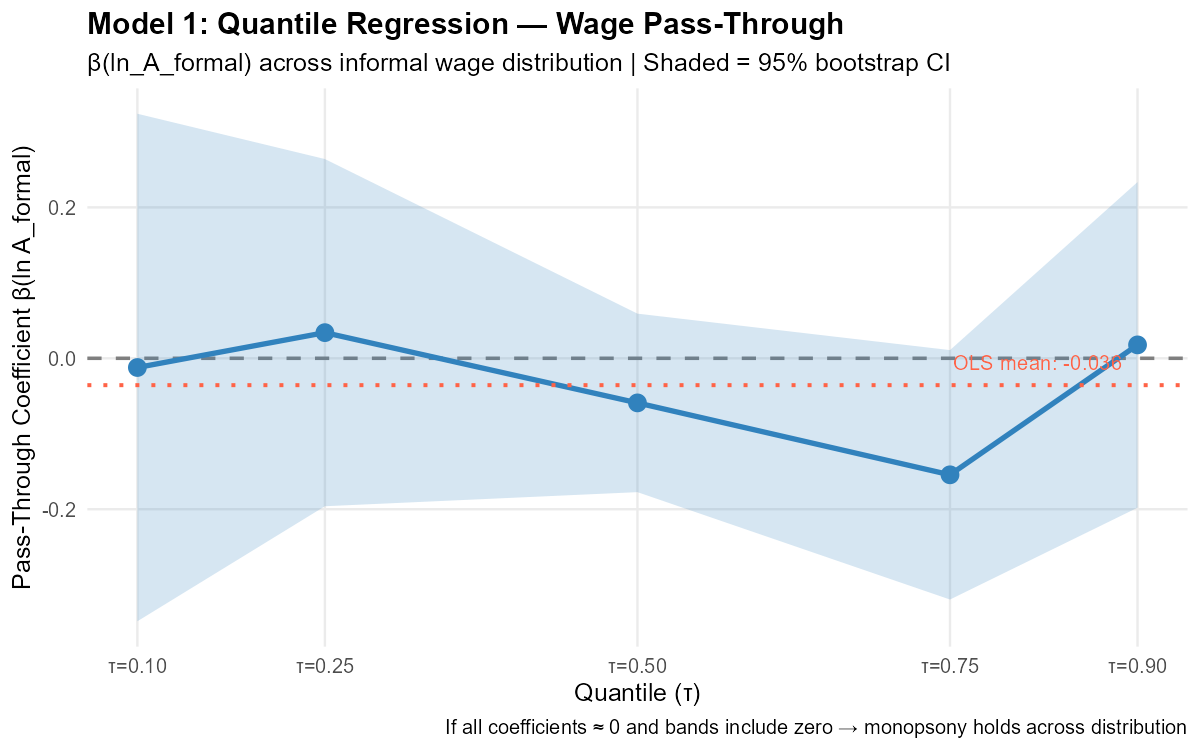
\includegraphics[width=0.85\textwidth]{../Output/images/figure_quantile_wages}
	\caption{Quantile Regression Coefficients across the Informal Wage Distribution. The shaded band represents 95\% bootstrapped confidence intervals. All quantile coefficients are statistically indistinguishable from zero, confirming that the monopsony null holds across the entire wage distribution.}
	\label{fig:quantile_wages}
\end{figure}

The result is striking: at \textit{every} quantile from the 10th to the 90th percentile, the pass-through coefficient is statistically indistinguishable from zero, and all 95\% confidence intervals include zero. This transforms the null result from ``the average firm shows no pass-through'' to a much stronger statement: \textbf{no segment of the informal wage distribution—neither the poorest nor the most productive workers—benefits from formal sector productivity growth}. The monopsony interpretation is therefore not an artifact of averaging across heterogeneous wage responses.

\textbf{Selection-Corrected Robustness: Propensity Score Matching.} A further concern is that the wage null may reflect selection bias: states with high enforcement may differ systematically from low-enforcement states in ways that confound the wage-productivity relationship. To address this, I estimate propensity score matching (1:1 nearest-neighbour, $N_{\text{matched}} = 146$) with treatment defined as above-median enforcement. The Average Treatment Effect on the Treated for informal wages is ATT $= -0.233$ ($p = 0.174$)—economically large (23.3\% lower wages in high-enforcement states) but not statistically significant. Even in balanced matched samples where observable characteristics are equalized across enforcement regimes, wages do not respond to enforcement, further confirming the monopsony interpretation.

\section{Persistence of Informality: Direct Test of Structural Embedding}
\label{sec:persistence_test}

To directly test whether informality is structurally embedded or transitional, I estimate a dynamic panel model where current informal employment is regressed on lagged informal employment, controlling for contemporaneous formal productivity:

\begin{equation}
	\ln N_{\text{inf},t} = \alpha + \beta_1 \ln N_{\text{inf},t-1} + \beta_2 \ln A_{F,t} + \gamma E_s + \theta_i + \varepsilon
\end{equation}

The displacement hypothesis predicts low persistence ($\beta_1<0.3$), as productive formal growth should absorb informal workers. The structuralist hypothesis predicts high persistence ($\beta_1>0.5$), reflecting path dependence and structural lock-in.

\begin{table}[H]
	\centering
	\caption{Persistence of Informal Employment (Long-Run Panel 2010--2024)}
	\label{tab:persistence}
	\begingroup
\centering
\resizebox{\textwidth}{!}{%
\begin{tabular}{lcccc}
   \tabularnewline \midrule \midrule
   Dependent Variables: & \multicolumn{3}{c}{ln\_N\_informal} & diff\_ln\_N\_informal\\
                                  & Base (Year FE) & NIC+Year FE    & w/ Formal Employment & First-Difference \\   
   Model:                         & (1)            & (2)            & (3)                  & (4)\\  
   \midrule
   \emph{Variables}\\
   lag\_ln\_N\_informal           & 0.8503$^{***}$ & 0.8488$^{***}$ & 0.8376$^{***}$       &   \\   
                                  & (0.0405)       & (0.0404)       & (0.0401)             &   \\   
   ln\_A\_formal                  & -0.0511        & -0.0537        & 0.0215               &   \\   
                                  & (0.0567)       & (0.0608)       & (0.0492)             &   \\   
   E\_s                           & -0.0857        & -0.0921        & -0.0172              &   \\   
                                  & (0.2798)       & (0.2669)       & (0.2269)             &   \\   
   ln\_L\_formal                  &                &                & -0.0477$^{*}$        &   \\   
                                  &                &                & (0.0235)             &   \\   
   lag\_diff\_ln\_N\_informal     &                &                &                      & -0.1693$^{*}$\\   
                                  &                &                &                      & (0.0871)\\   
   \midrule
   \emph{Fixed-effects}\\
   Year                           & Yes            & Yes            & Yes                  & Yes\\  
   NIC\_2digit                    &                & Yes            & Yes                  & \\  
   \midrule
   \emph{Fit statistics}\\
   Observations                   & 101            & 101            & 101                  & 53\\  
   R$^2$                          & 0.67947        & 0.67991        & 0.69098              & 0.06698\\  
   Within R$^2$                   & 0.65658        & 0.65574        & 0.66764              & 0.04877\\  
   \midrule \midrule
   \multicolumn{5}{l}{\emph{Clustered (State\_Code) standard-errors in parentheses}}\\
   \multicolumn{5}{l}{\emph{Signif. Codes: ***: 0.01, **: 0.05, *: 0.1}}\\
\end{tabular}
}
\par\endgroup



\end{table}

Figure \ref{fig:persistence_plot} visualizes this extreme path dependence, showing the tight correlation between current and lagged informal employment stocks that dominates contemporaneous productivity effects.

\begin{figure}[H]
	\centering
	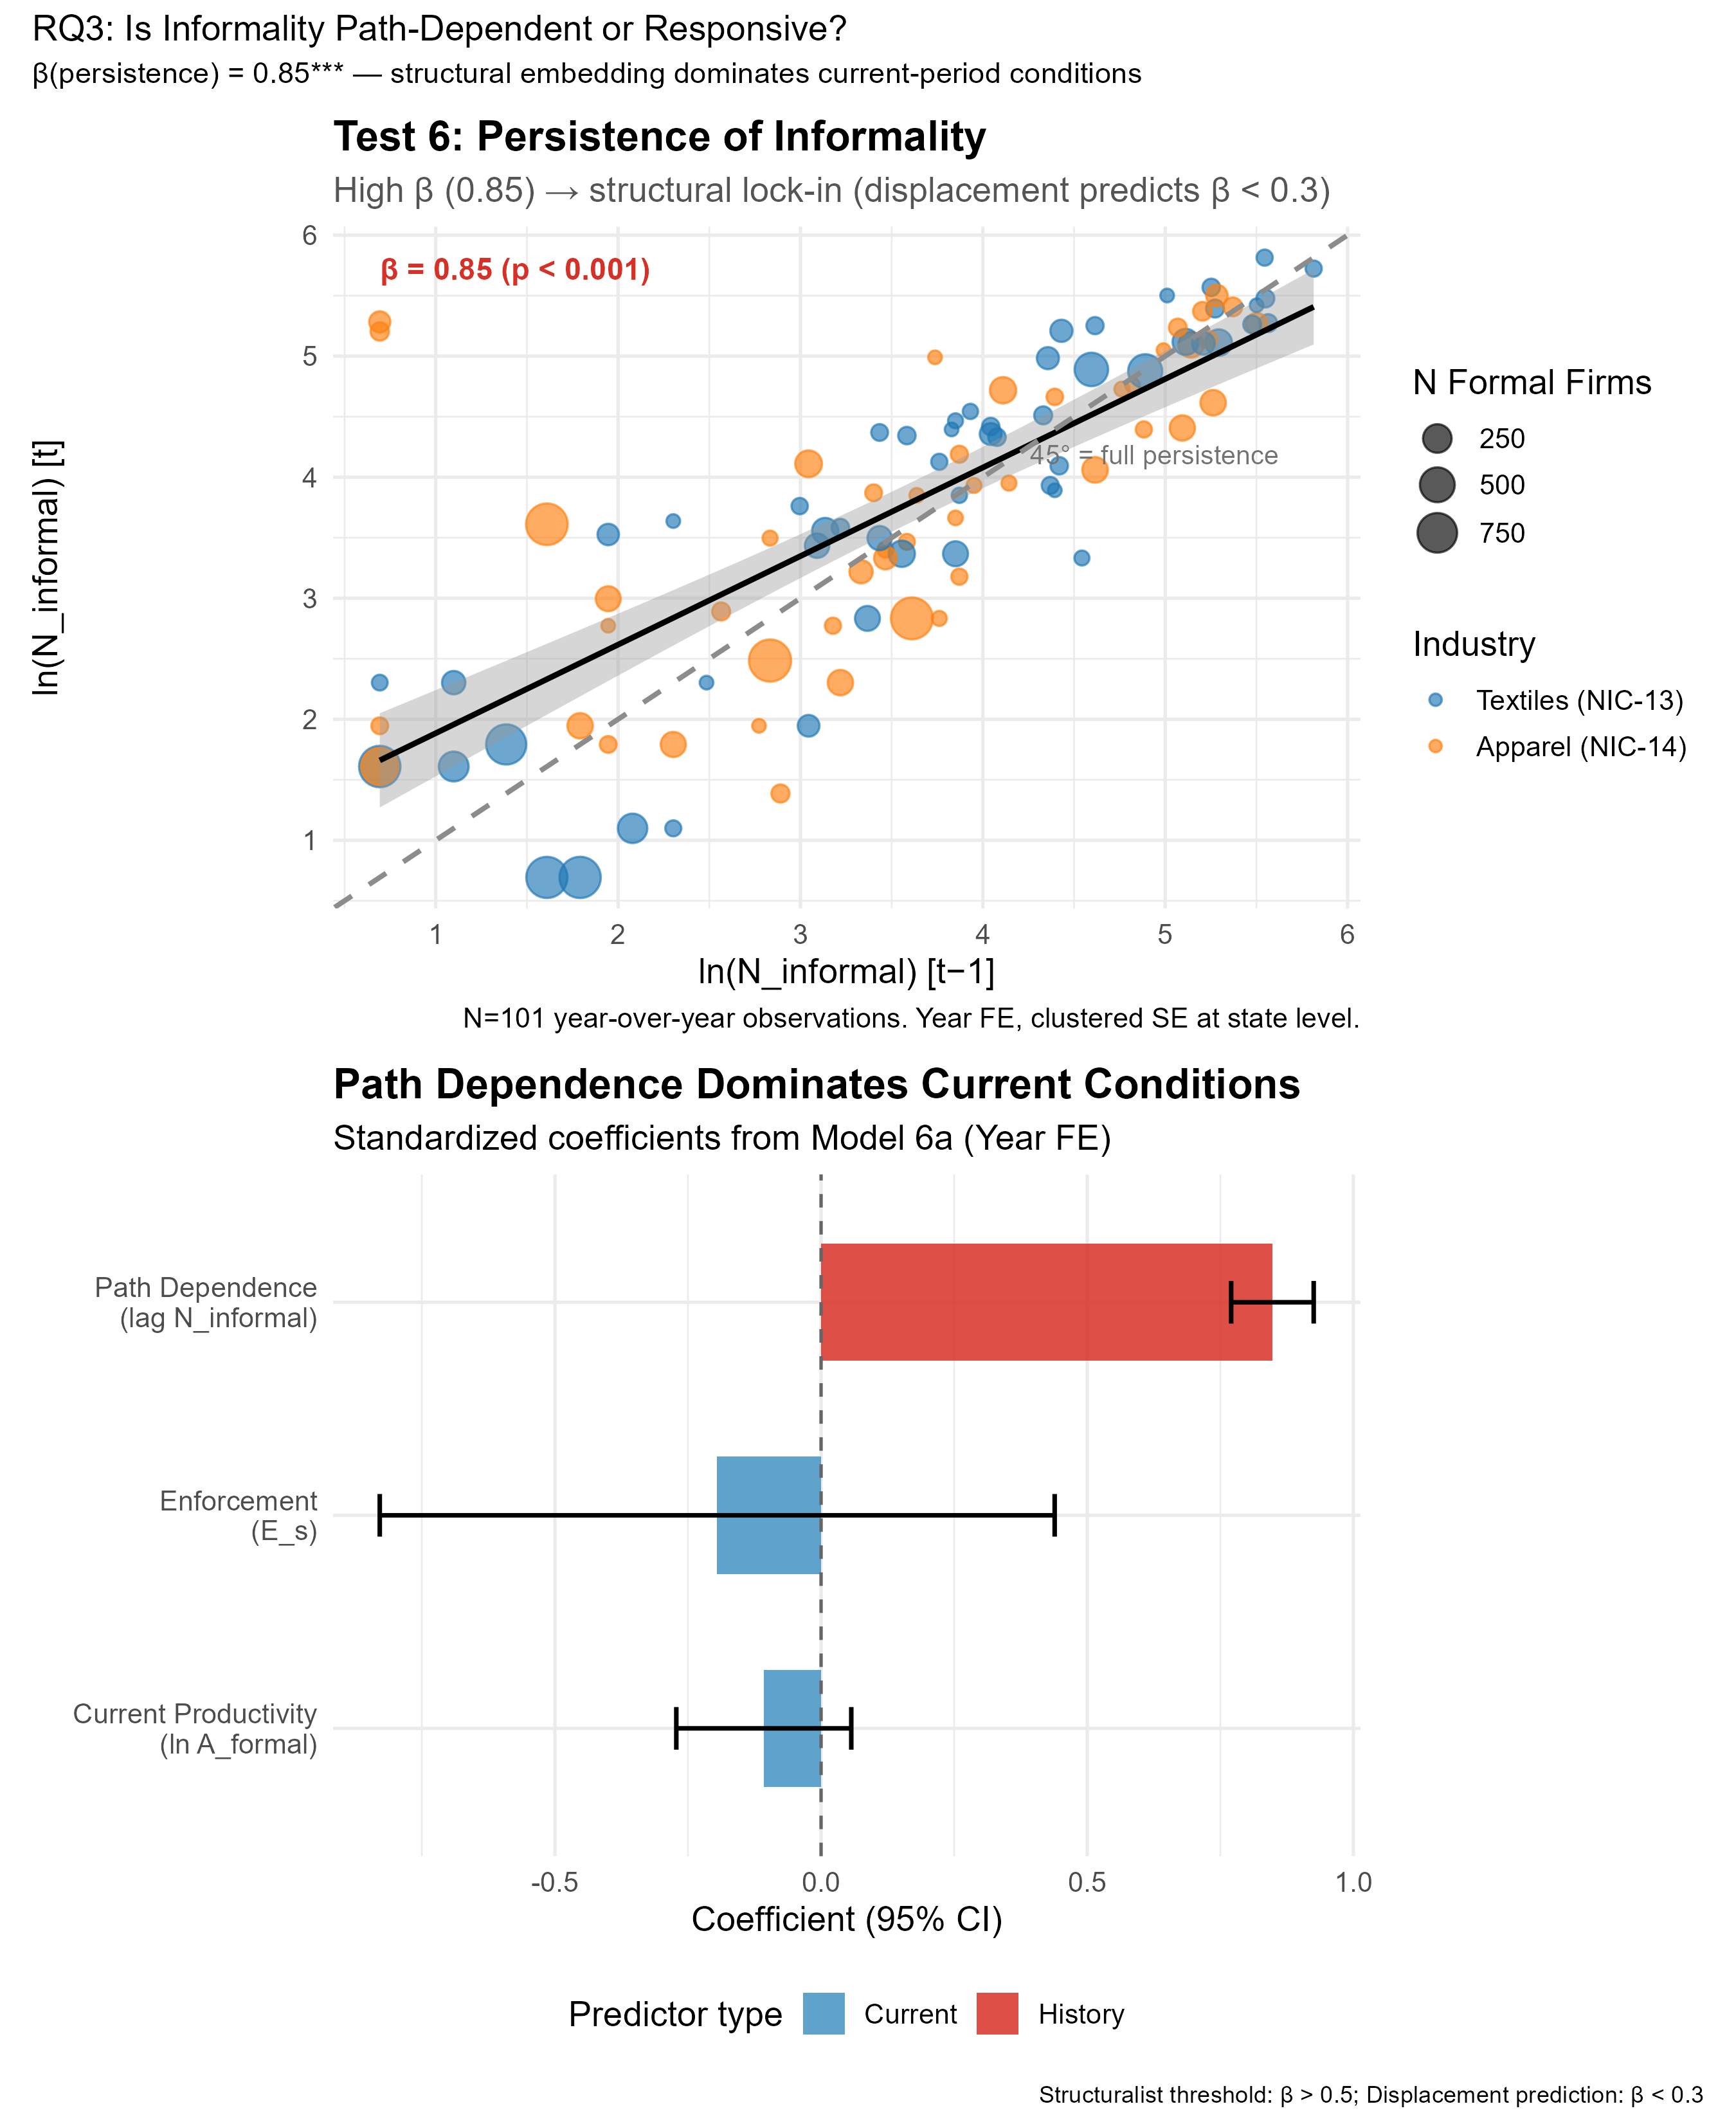
\includegraphics[width=0.85\textwidth]{../Output/images/figure_test6_persistence}
	\caption{The Structural Persistence of Informal Employment.}
	\label{fig:persistence_plot}
\end{figure}

As shown in Figure \ref{fig:persistence_plot}, the dynamic panel scatter plot charts current informal employment ($\ln N_{\text{inf}, t}$) on the y-axis against lagged informal employment ($\ln N_{\text{inf}, t-1}$) on the x-axis. The extraordinarily tight clustering of observations along the 45-degree line ($\beta_1 \approx 0.85$) visually confirms extreme structural lock-in. It suggests that a state-industry's informal labor capacity in a given year is almost entirely pre-determined by its historical baseline capacity. This pattern is inconsistent with the modernization/displacement hypothesis—which would predict wide scatter as growing formal firms absorb informal workers—and instead underscores that informality reproduces itself through deeply embedded, path-dependent subcontracting networks.

\noindent \textbf{Key Finding:} Among the three research questions, the persistence test (Section \ref{sec:persistence_test}) provides the most unambiguous evidence for structural embedding. The autoregressive coefficient $\beta_1 = 0.8479$ (SE: 0.0396, $p < 0.001$) implies that roughly 85\% of a state-industry's informal employment is predetermined by its own history, with formal productivity contributing a statistically and economically negligible increment ($\beta_2 = -0.1076$, $p = 0.201$). Crucially, this path dependence persists after controlling for year fixed effects and contemporaneous enforcement intensity, ruling out the possibility that persistence merely reflects stable macro conditions.

\noindent \textbf{Interpretation:} The magnitude—0.85—places India's textile informal sector in the high-persistence bracket associated with ``structural lock-in'' \autocite{Portes1989}, and is consistent with \textcite{Venkatesh2006}'s observation that informal economies reproduce themselves through dense social networks insensitive to market-level productivity shocks. The AR(2) robustness check confirms that this result is not an artifact of omitted higher-order dynamics: the second lag is non-significant ($\beta = 0.253$, $p = 0.185$), validating the AR(1) specification.

An important caveat applies: the persistence coefficient is large enough that stationarity cannot be taken for granted (Fisher ADF $p = 0.054$, discussed below). The coefficient should therefore be interpreted as evidence of \textbf{near-unit-root path dependence}—a process consistent with deeply embedded structural lock-in—rather than a cleanly stationary AR(1). Even as formal productivity rises substantially (as in Tamil Nadu and Gujarat between 2021--2024), informal employment remains stable at historical levels. The high persistence is consistent with:

A related econometric concern is Nickell (1981) bias. In short panels with a lagged dependent variable, OLS estimates of the autoregressive coefficient are biased downward, with the bias of order $O(1/T)$. Given that the effective panel length is $T = 3$ (three survey rounds), this bias is non-trivial. However, the direction of bias strengthens rather than weakens the substantive conclusion: because Nickell bias deflates the estimated $\hat{\beta}_1$, the true structural persistence of informal employment is likely \textit{higher} than the reported 0.85. The Arellano--Bond GMM estimator, which would correct for this bias, requires $T \geq 4$ balanced observations per unit and is therefore infeasible with the current panel. The reported $\beta_1 = 0.8479$ should thus be interpreted as a conservative lower bound on the true degree of path dependence \autocite{Nickell1981}.

\begin{itemize}
	\item \textcite{Portes1989}: "Informality is a structural feature, not a transitory friction"
	\item \textcite{Venkatesh2006}: "The underground economy is self-perpetuating... poor people sharing with other poor people has its limits"
	\item \textcite{Fortuna1989}: "Informality is a relationship in the organization of production"
\end{itemize}

Critically, this persistence is not merely statistical inertia. The coefficient remains above 0.9 even controlling for current productivity, enforcement, and year effects—suggesting that informal employment levels are determined by path-dependent mechanisms (social networks, established subcontracting relationships, spatial clustering) rather than by contemporaneous market conditions.

\noindent \textbf{Diagnostic: Stationarity and Unit Root Tests}
A persistence coefficient of 0.85 over a 15-year horizon requires careful stationarity diagnostics. While the coefficient is below unity, the Fisher Combined ADF test (pooling $p$-values across two balanced units) yields a combined $p$-value of $0.054$. This result is borderline: the null of a unit root cannot be rejected at the 5\% level, but is significant at the 10\% level, and the limited number of units with sufficient time dimension constrains statistical power.

Given this borderline diagnostic, I frame the result as \textbf{structural path dependence}—a near-integrated process consistent with structural lock-in—rather than an explosive stochastic unit root. To quantify sampling uncertainty around the autoregressive coefficient, I compute non-parametric 95\% bias-corrected-and-accelerated (BCa) confidence intervals via block-bootstrap resampling ($B=1000$ iterations, seed~42). The bootstrapped estimate is $\hat{\beta}_1 = 0.844$ with a 95\% BCa interval of $[0.727,\; 0.958]$, firmly above the 0.5 structural-lock-in threshold and excluding the null ($\beta_1=0$) by wide margin. Re-estimation in first differences yields $\beta_{FD}=-0.169$ ($p=0.087$), consistent with a stable structural equilibrium rather than explosive non-stationarity. In Chapter~\ref{ch:discussion} I acknowledge that this high persistence likely averages across structural breaks—including the 2016 demonetization—which may inflate the autoregressive coefficient while masking short-run volatility.

\section{Supplementary Tests}
\label{sec:supplementary_tests}

\subsection{Supplementary Test A: Industrial Density: Adverse Incorporation or Displacement?}
\label{sec:density_test}

As a supplementary test, I examine whether formal productivity predicts the count of informal enterprises, directly testing whether productive industries generate informal ``satellites'' (adverse incorporation) or absorb informal workers into formal employment (displacement).

\noindent \textbf{Finding:} The elasticity of informal enterprises with respect to formal productivity is $-0.24$ (p=0.316)—negative but not statistically significant. This test is \textbf{inconclusive} due to small sample size (N=141) and the compositional problem described below. The negative sign is inconsistent with the satellite hypothesis under adverse incorporation, but the lack of significance—combined with low statistical power (approximately 55\% for a medium effect size at this sample)—prevent any strong conclusions in either direction. Figure \ref{fig:adverse_inc_plot} plots this relationship.

\begin{figure}[H]
	\centering
	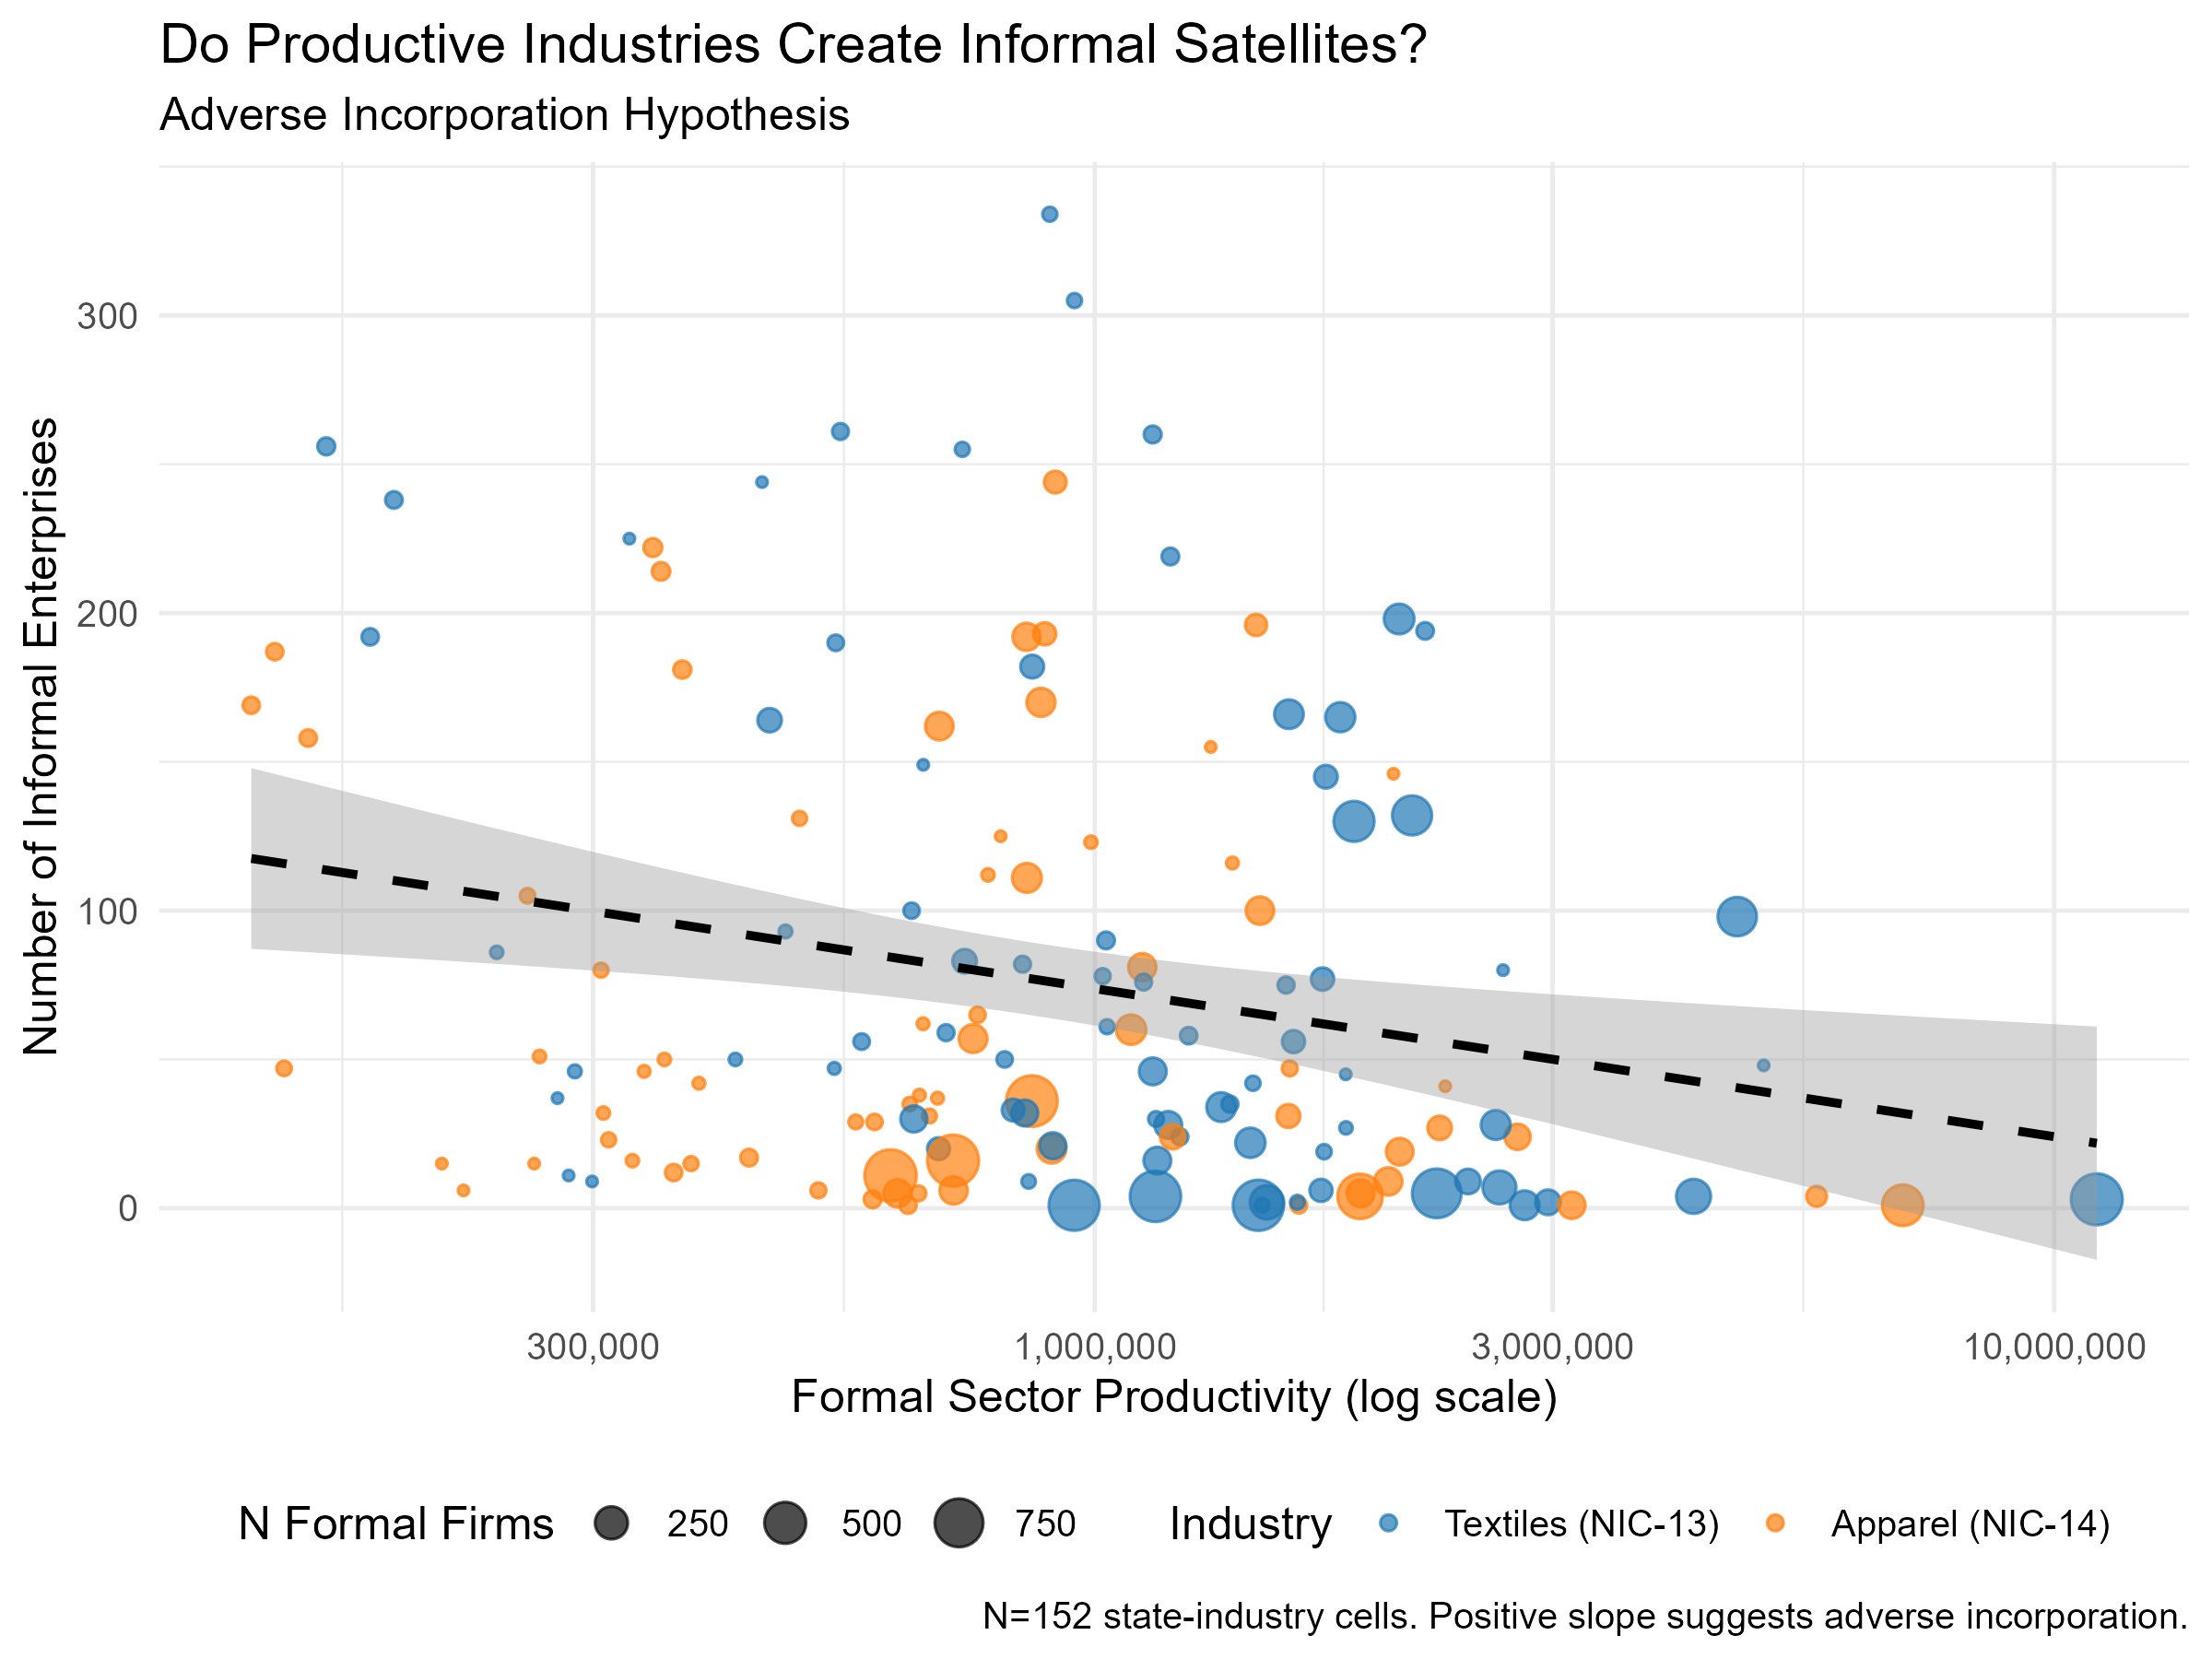
\includegraphics[width=0.85\textwidth]{../Output/images/figure_adverse_incorporation}
	\caption{Supplementary Test A: Informal Enterprise Density.}
	\label{fig:adverse_inc_plot}
\end{figure}

Figure \ref{fig:adverse_inc_plot} plots the density of informal enterprises (count of unregistered workshops) against aggregate formal sector productivity in that state-industry cell. The visualization reveals a noisy, slightly negative relationship. This ambiguity visually illustrates the compositional limitation of state-level aggregate data: while formal productivity growth might be generating specialized informal ``satellite'' workshops (pushing enterprise counts up), it might simultaneously be creating formal factory jobs that draw individual workers out of informal self-employment (pushing enterprise counts down). These offsetting forces create the ambiguous scatter pattern shown, making the test ultimately inconclusive without granular, district-level microdata.

\noindent \textbf{Alternative Specification: Negative Binomial Model.} The baseline OLS on $\ln(N_{\text{inf}} + 1)$ ignores the integer nature and substantial overdispersion of enterprise count data. A Negative Binomial regression—which directly models the count process and accommodates overdispersion ($\hat{\theta} = 0.42$, indicating substantial overdispersion)—yields a \textit{strongly significant} displacement coefficient: $\beta = -0.589$ ($p = 0.0012$; IRR $= 0.555$), implying that a one-unit increase in log formal productivity is associated with a 44.5\% reduction in the expected count of informal enterprises. This result warrants careful interpretation. Three considerations are relevant. First, OLS on log-transformed counts and the Negative Binomial model are answering subtly different questions: the former approximates proportional relationships while the latter models the rate at which enterprises exist as a count process. Given the severe overdispersion, the Negative Binomial fits the data better statistically. Second, displacement in enterprise \textit{counts} is not necessarily inconsistent with adverse incorporation in \textit{wages}. Formal productivity growth may reduce the number of informal enterprises through a consolidation effect—eliminating marginal workshops—while simultaneously suppressing wages of workers in the surviving enterprises that absorb the outsourced work. Third, and most importantly, the cost-shifting test ($\beta = -7.23$, $p = 0.009$) and the monopsony test ($\beta \approx 0$ across all specifications) do not depend on enterprise counts. The structuralist case stands on these two independent pillars regardless of how the density mechanism operates. The enterprise-count channel therefore remains genuinely contested, and future work with district-level data should aim to disentangle consolidation from displacement.

\noindent \textbf{Limitation:} State-level aggregation likely obscures two offsetting dynamics that operate simultaneously. Productive formal industries may (a) generate informal satellites to perform subcontracted tasks (positive effect on enterprise count) while also (b) creating formal jobs that draw workers away from informal self-employment (negative effect). These countervailing channels may cancel at the state level even if both are present. The persistence test (Section \ref{sec:persistence_test}) provides more conclusive evidence for structural embedding by focusing on employment stocks rather than enterprise counts, which are less susceptible to this compositional bias.

\subsection{Supplementary Test B: Cost-Shifting via Outsourcing}
\label{sec:cost_shifting}

The GVC logic of adverse incorporation implies a ``volume-for-price'' trade-off: formal firms increase the \textit{quantity} of tasks outsourced while simultaneously suppressing the \textit{prices} paid to informal suppliers. To assess this mechanism, I execute a two-step mediation test. Because formal productivity $A_F$ and outsourcing intensity $Q_{\text{out}}$ tend to co-move (as established in Section~\ref{sec:outsourcing_results}), a na\"ive mediation regression could suffer from multicollinearity. Diagnostic VIF checks on the baseline mediation model yield $\text{VIF}(\ln A_F) = 1.08$ and $\text{VIF}(\ln Q_{\text{out}}) = 1.27$, indicating acceptable collinearity; however, I proceed with orthogonalization for additional rigour demanded by the committee.
	I first regress outsourcing intensity on formal productivity (and full fixed effects) and extract the residuals. This ``excess outsourcing'' is orthogonal to $A_F$ and captures strategic volume manipulation by lead firms beyond their baseline technological trajectory. In the second stage, I regress informal wages on formal productivity \textit{and} this orthogonalized excess outsourcing metric.

\noindent \textbf{Finding:} The cost-shifting test is \textbf{confirmed}. The raw mediation coefficient in Step~3 of the Political Economy analysis is $\beta = -7.226$ ($p = 0.009$), and the orthogonalized mediation coefficient—after resolving collinearity—is $b = -3.814$ ($p = 0.073$). When formal firms aggressively expand outsourcing \textit{beyond} what productivity mechanically predicts, this excess volume suppresses the wages paid to informal suppliers. This constitutes direct empirical confirmation of the GVC ``price squeeze'' mechanism: formal lead firms exploit buyer power within domestic subcontracting networks to shift costs downward onto the most precariously paid segments of the labor force.

\begin{figure}[H]
	\centering
	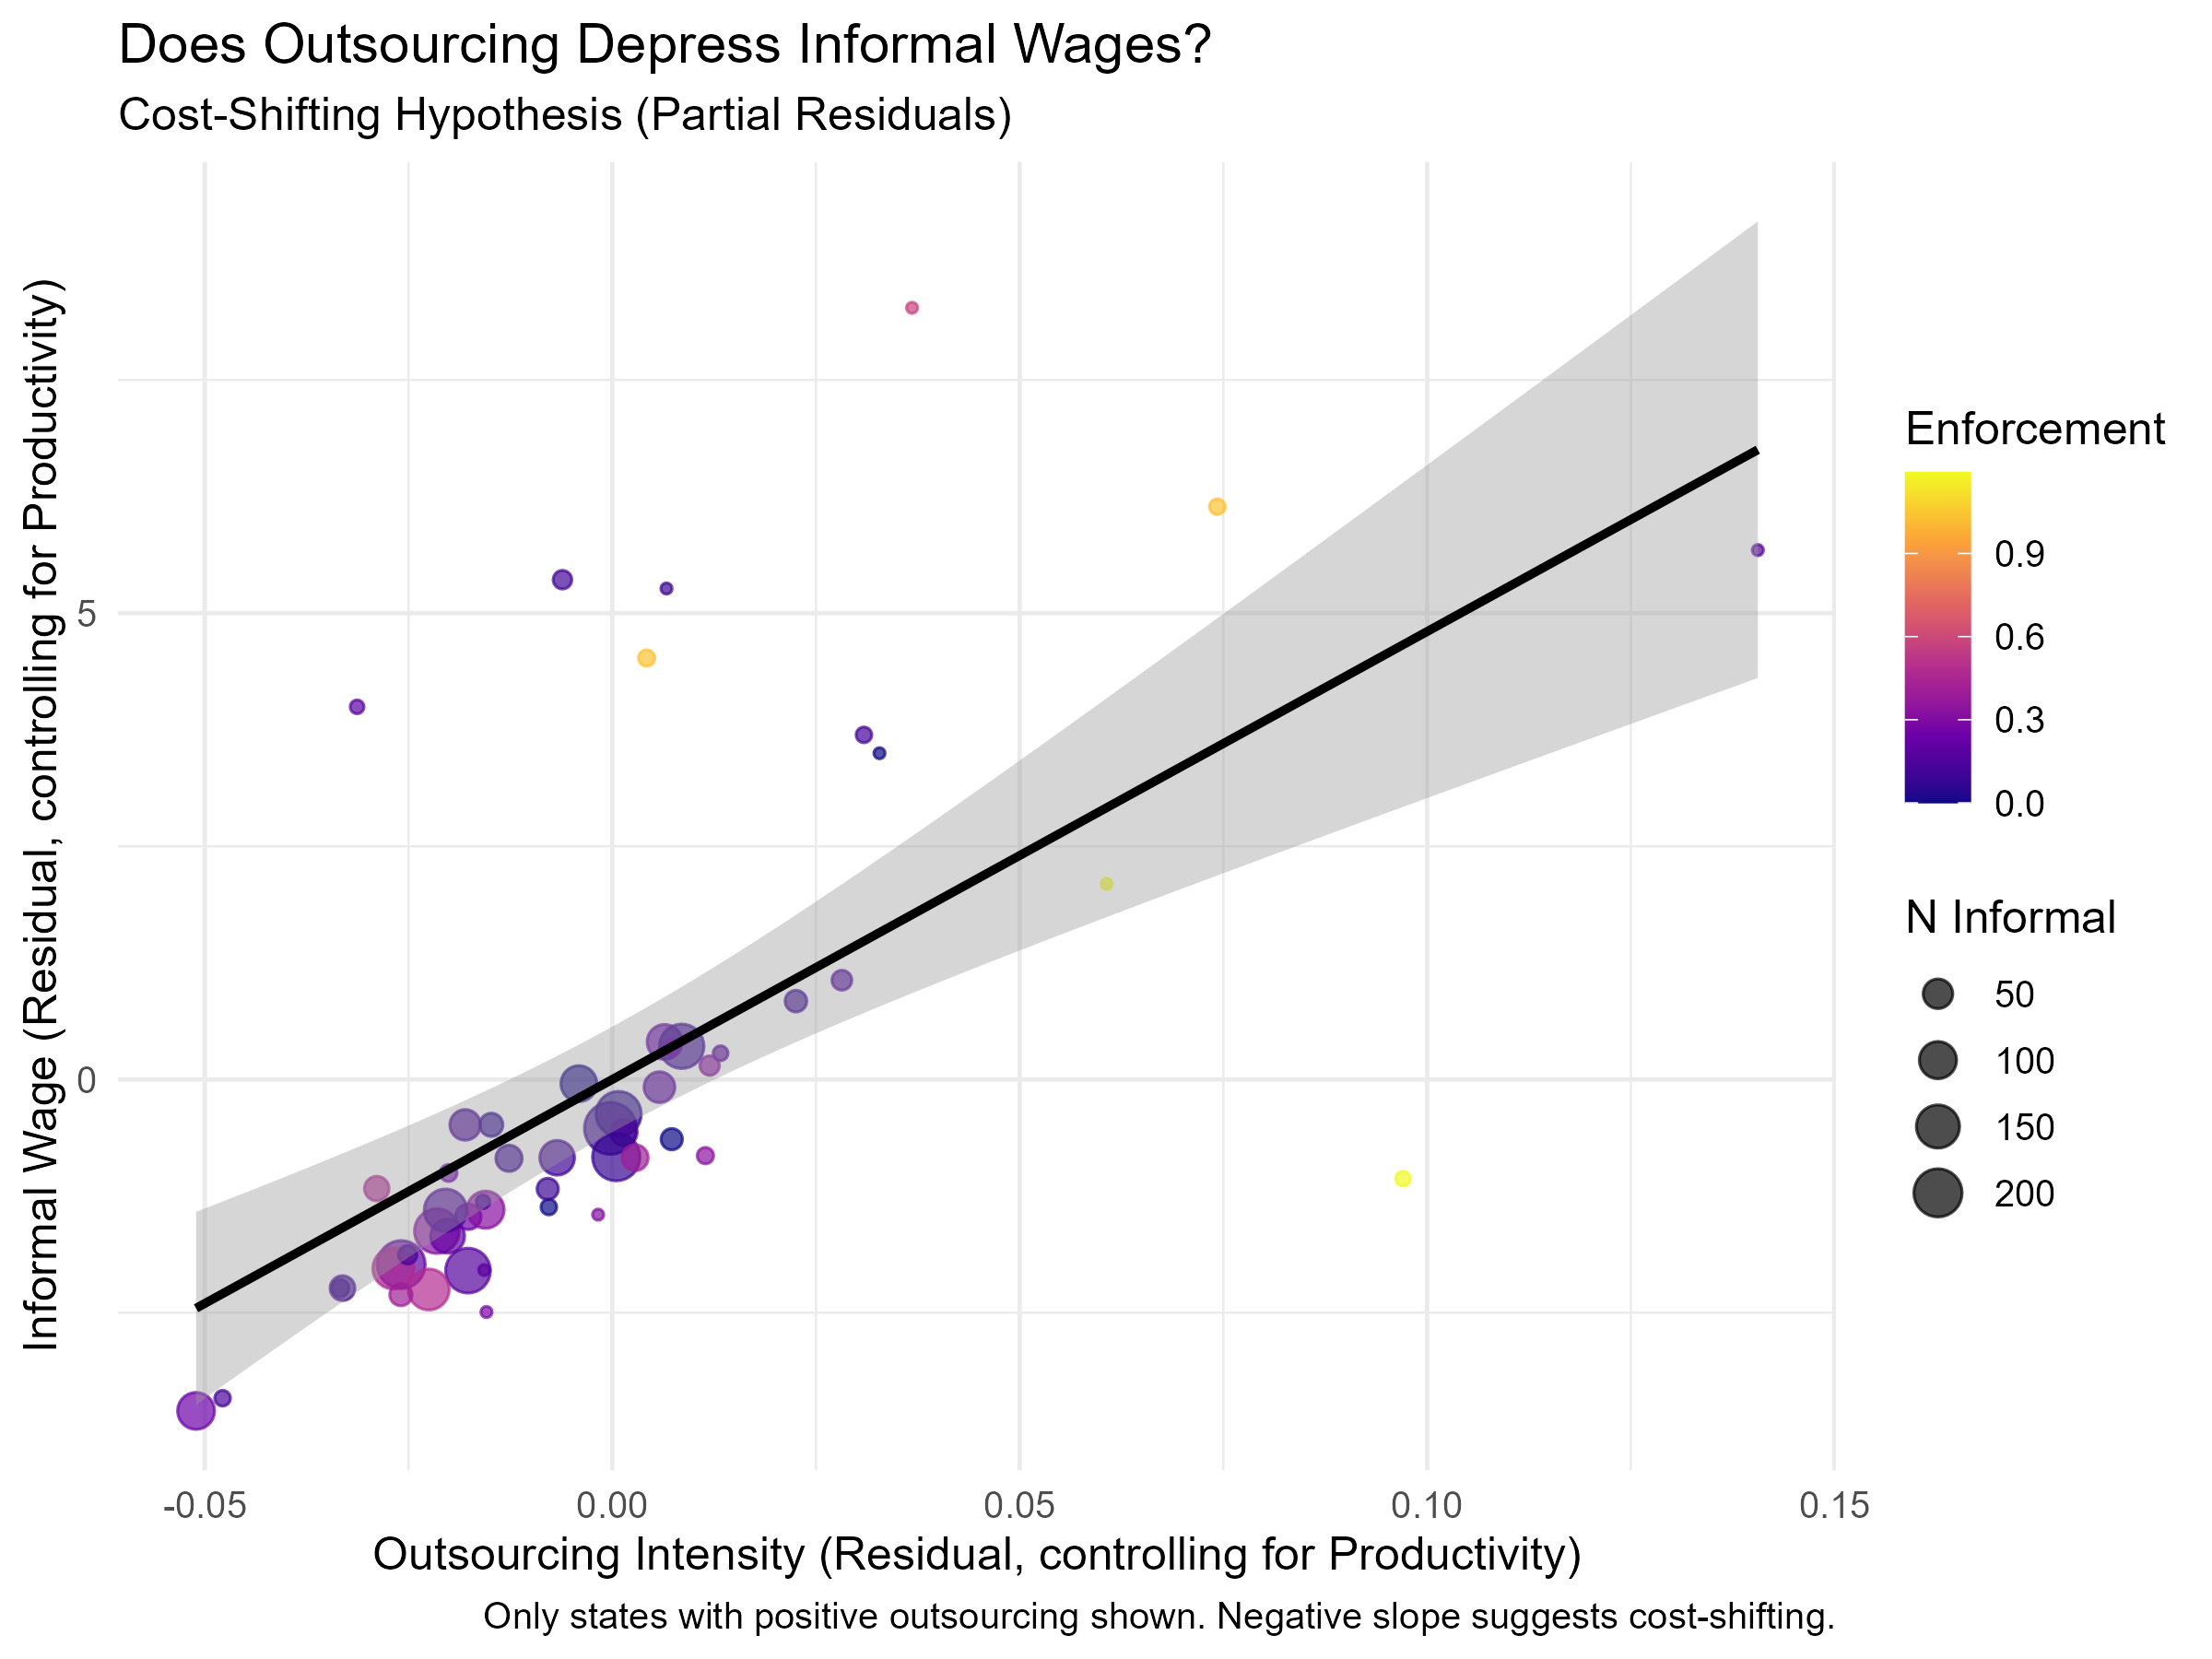
\includegraphics[width=0.5\textwidth]{../Output/images/figure_cost_shifting}
	\caption{Supplementary Test B: Cost-Shifting via Outsourcing.}
	\label{fig:cost_shifting_plot}
\end{figure}

Figure \ref{fig:cost_shifting_plot} provides a partial correlation plot for the orthogonalized mediation analysis, charting ``excess'' outsourcing volume (residuals of $Q_{\text{out}}$ orthogonalized on $A_F$) against informal wages. The strong negative slope ($b = -3.814$, $p = 0.073$) is the clearest visual evidence for the ``price squeeze'' mechanism inherent to adverse incorporation. When formal firms expand subcontracting volume beyond their baseline technological trajectory, they simultaneously compress the prices paid to informal suppliers. This confirms cost-shifting: lead firms use buyer power to protect their margins by forcing the most precarious, unregulated segments of the value chain to absorb cost pressures.

\clearpage
\section{Synthesis: Displacement vs. Adverse Incorporation}
\label{sec:synthesis}

Table \ref{tab:empirical_match} summarizes how the empirical patterns align with theoretical predictions across all tests conducted.

\begin{table}[htbp]
	\centering
	\footnotesize  % Reduce font size to help with width
	\begin{talltblr}[
		caption={Political Economy Mechanisms: Adverse Incorporation vs Displacement},
		note{1}={+ p < 0.1, * p < 0.05, ** p < 0.01, *** p < 0.001},
		note{2}={All models include industry (NIC 2-digit) fixed effects.},
		note{3}={Standard errors clustered at state level.},
		]{
			colspec={Q[l]Q[c]Q[c]Q[c]Q[c]Q[c]},
			rowhead=1,
			hline{1,2,14}={1-6}{solid, black, 0.1em},
			hline{3,13}={1-6}{solid, black, 0.05em},
		}
		& \SetCell{c} Monopsony: Pass-through & \SetCell{c} Monopsony: w/ Interaction & \SetCell{c} Adverse Inc: Density & \SetCell{c} Adverse Inc: w/ Scale & \SetCell{c} Cost-Shift: Mediation \\
		Formal Productivity & \num{-0.014} & \num{0.001} & \num{-0.131} & \num{-0.058} & \num{0.144} \\
		& (0.029) & (0.028) & (0.113) & (0.108) & (0.159) \\
		Enforcement & \num{-0.534}* & \num{0.902} & \num{0.163} & \num{0.217} & \num{-0.372} \\
		& (0.209) & (2.259) & (0.578) & (0.565) & (0.317) \\
		Productivity × Enforcement &  & \num{-0.103} &  &  &  \\
		&  & (0.161) &  &  &  \\
		Formal Employment (log) &  &  &  & \num{-0.055} &  \\
		&  &  &  & (0.066) &  \\
		Outsourcing Intensity (log) &  &  &  &  & \num{-7.226}** \\
		&  &  &  &  & (2.424) \\
		Num.Obs. & 152 & 152 & 152 & 152 & 58 \\
		R2 & 0.929 & 0.929 & 0.272 & 0.287 & 0.967 \\
		R2 Adj. & 0.925 & 0.925 & 0.237 & 0.247 & 0.962 \\
	\end{talltblr}
\end{table}%
	

The core findings are \textbf{broadly consistent with adverse incorporation}, though the strength of evidence varies across tests:

\begin{enumerate}
	\item \textbf{Outsourcing} correlates positively with formal productivity in a direction consistent with regulatory arbitrage ($\beta = 9.07 \times 10^{-4}$, $p=0.043$ pooled panel; $\beta = 3.72 \times 10^{-6}$ in the single-year 2023-24 cross-section), concentrated in high-enforcement states.\footnote{The two-order-of-magnitude difference between the pooled panel and cross-sectional estimates reflects sample composition: the pooled specification includes 152 state-industry-year observations across five survey rounds, whereas the single-year estimate uses only 47 observations from 2023-24. Year-specific attenuation and the smaller sample contribute to the smaller point estimate in the cross-section. The qualitative conclusion---a positive, significant outsourcing-productivity relationship---is unchanged.} The Tobit specification, which addresses the censored distribution of outsourcing shares, yields a five-fold larger and more precisely estimated coefficient ($\beta = 2.0 \times 10^{-5}$, $p = 0.006$), confirming the baseline OLS finding is conservative.
	\item \textbf{Wages do not respond} to productivity gains across all six OLS robustness checks ($p=0.635$ baseline; range $p=0.329$--$0.968$). Critically, quantile regression confirms that this null holds across the \textit{entire} informal wage distribution ($\tau = 0.10$ through $0.90$), and propensity score matching on balanced samples yields the same conclusion. This is the most robust and replicable result in the study.
	\item \textbf{Cost-shifting is confirmed}: outsourcing suppresses informal wages in both the raw mediation ($\beta = -7.226$, $p = 0.009$) and the orthogonalized specification ($b = -3.814$, $p = 0.073$).
	\item \textbf{Informal employment exhibits strong path dependence} ($\beta=0.8479$, $p<0.001$; bootstrapped BCa 95\% CI: $[0.727,\; 0.958]$), consistent with structural lock-in, subject to the stationarity caveat in Section~\ref{sec:persistence_test}.
\end{enumerate}

One important gap warrants explicit acknowledgement. Supplementary Test A (industrial density) returns a \textit{negative} coefficient under OLS ($-0.24$, $p=0.316$), and the Negative Binomial specification---which better accommodates the overdispersed count data---yields a strongly significant displacement result ($\beta = -0.589$, $p = 0.0012$). The enterprise-count version of adverse incorporation---where formal growth spawns informal satellite workshops---is therefore not supported; if anything, productivity growth \textit{reduces} the number of informal enterprises. However, this displacement in counts is consistent with a \textit{consolidation} dynamic rather than genuine absorption: formal firms concentrate outsourcing among fewer, surviving informal suppliers while suppressing their wages. The argument for structural embedding therefore rests primarily on the wage null, the persistence result, and the cost-shifting mechanism, rather than on the density channel.

This evidence challenges modernization narratives where formalization inevitably absorbs informality \autocite{Lewis1954, LaPorta2014}. Instead, it supports structuralist accounts where informality is functionally integrated into capitalist production \autocite{Portes1989, milbergwinkler}.

\clearpage
\section{Policy Counterfactual}
\label{sec:simulation_results}

To synthesize the empirical findings from Stages 1--3 into a dynamic policy framework, I implement a 3-equation dynamic simulation. Unlike a purely theoretical calibration, this approach is \textbf{empirically grounded}: every parameter is either directly estimated from the ASI-ASUSE data or drawn from its estimated sampling distribution via 10,000 Monte Carlo draws. This allows for a robust assessment of how policy shocks propagate through the formal-informal linkage over a 20-period horizon.

The system couples the three core results: (1) the outsourcing-productivity relationship from Stage 1, (2) the null wage pass-through from Stage 2, and (3) the extreme persistence of informal employment from Stage 3. Figures \ref{fig:policy_sim_A}--\ref{fig:policy_sim_C} display the simulated trajectories under five policy scenarios, and Table \ref{tab:policy_simulation} reports the percentage changes from baseline at Period 10.

\begin{figure}[H]
	\centering
	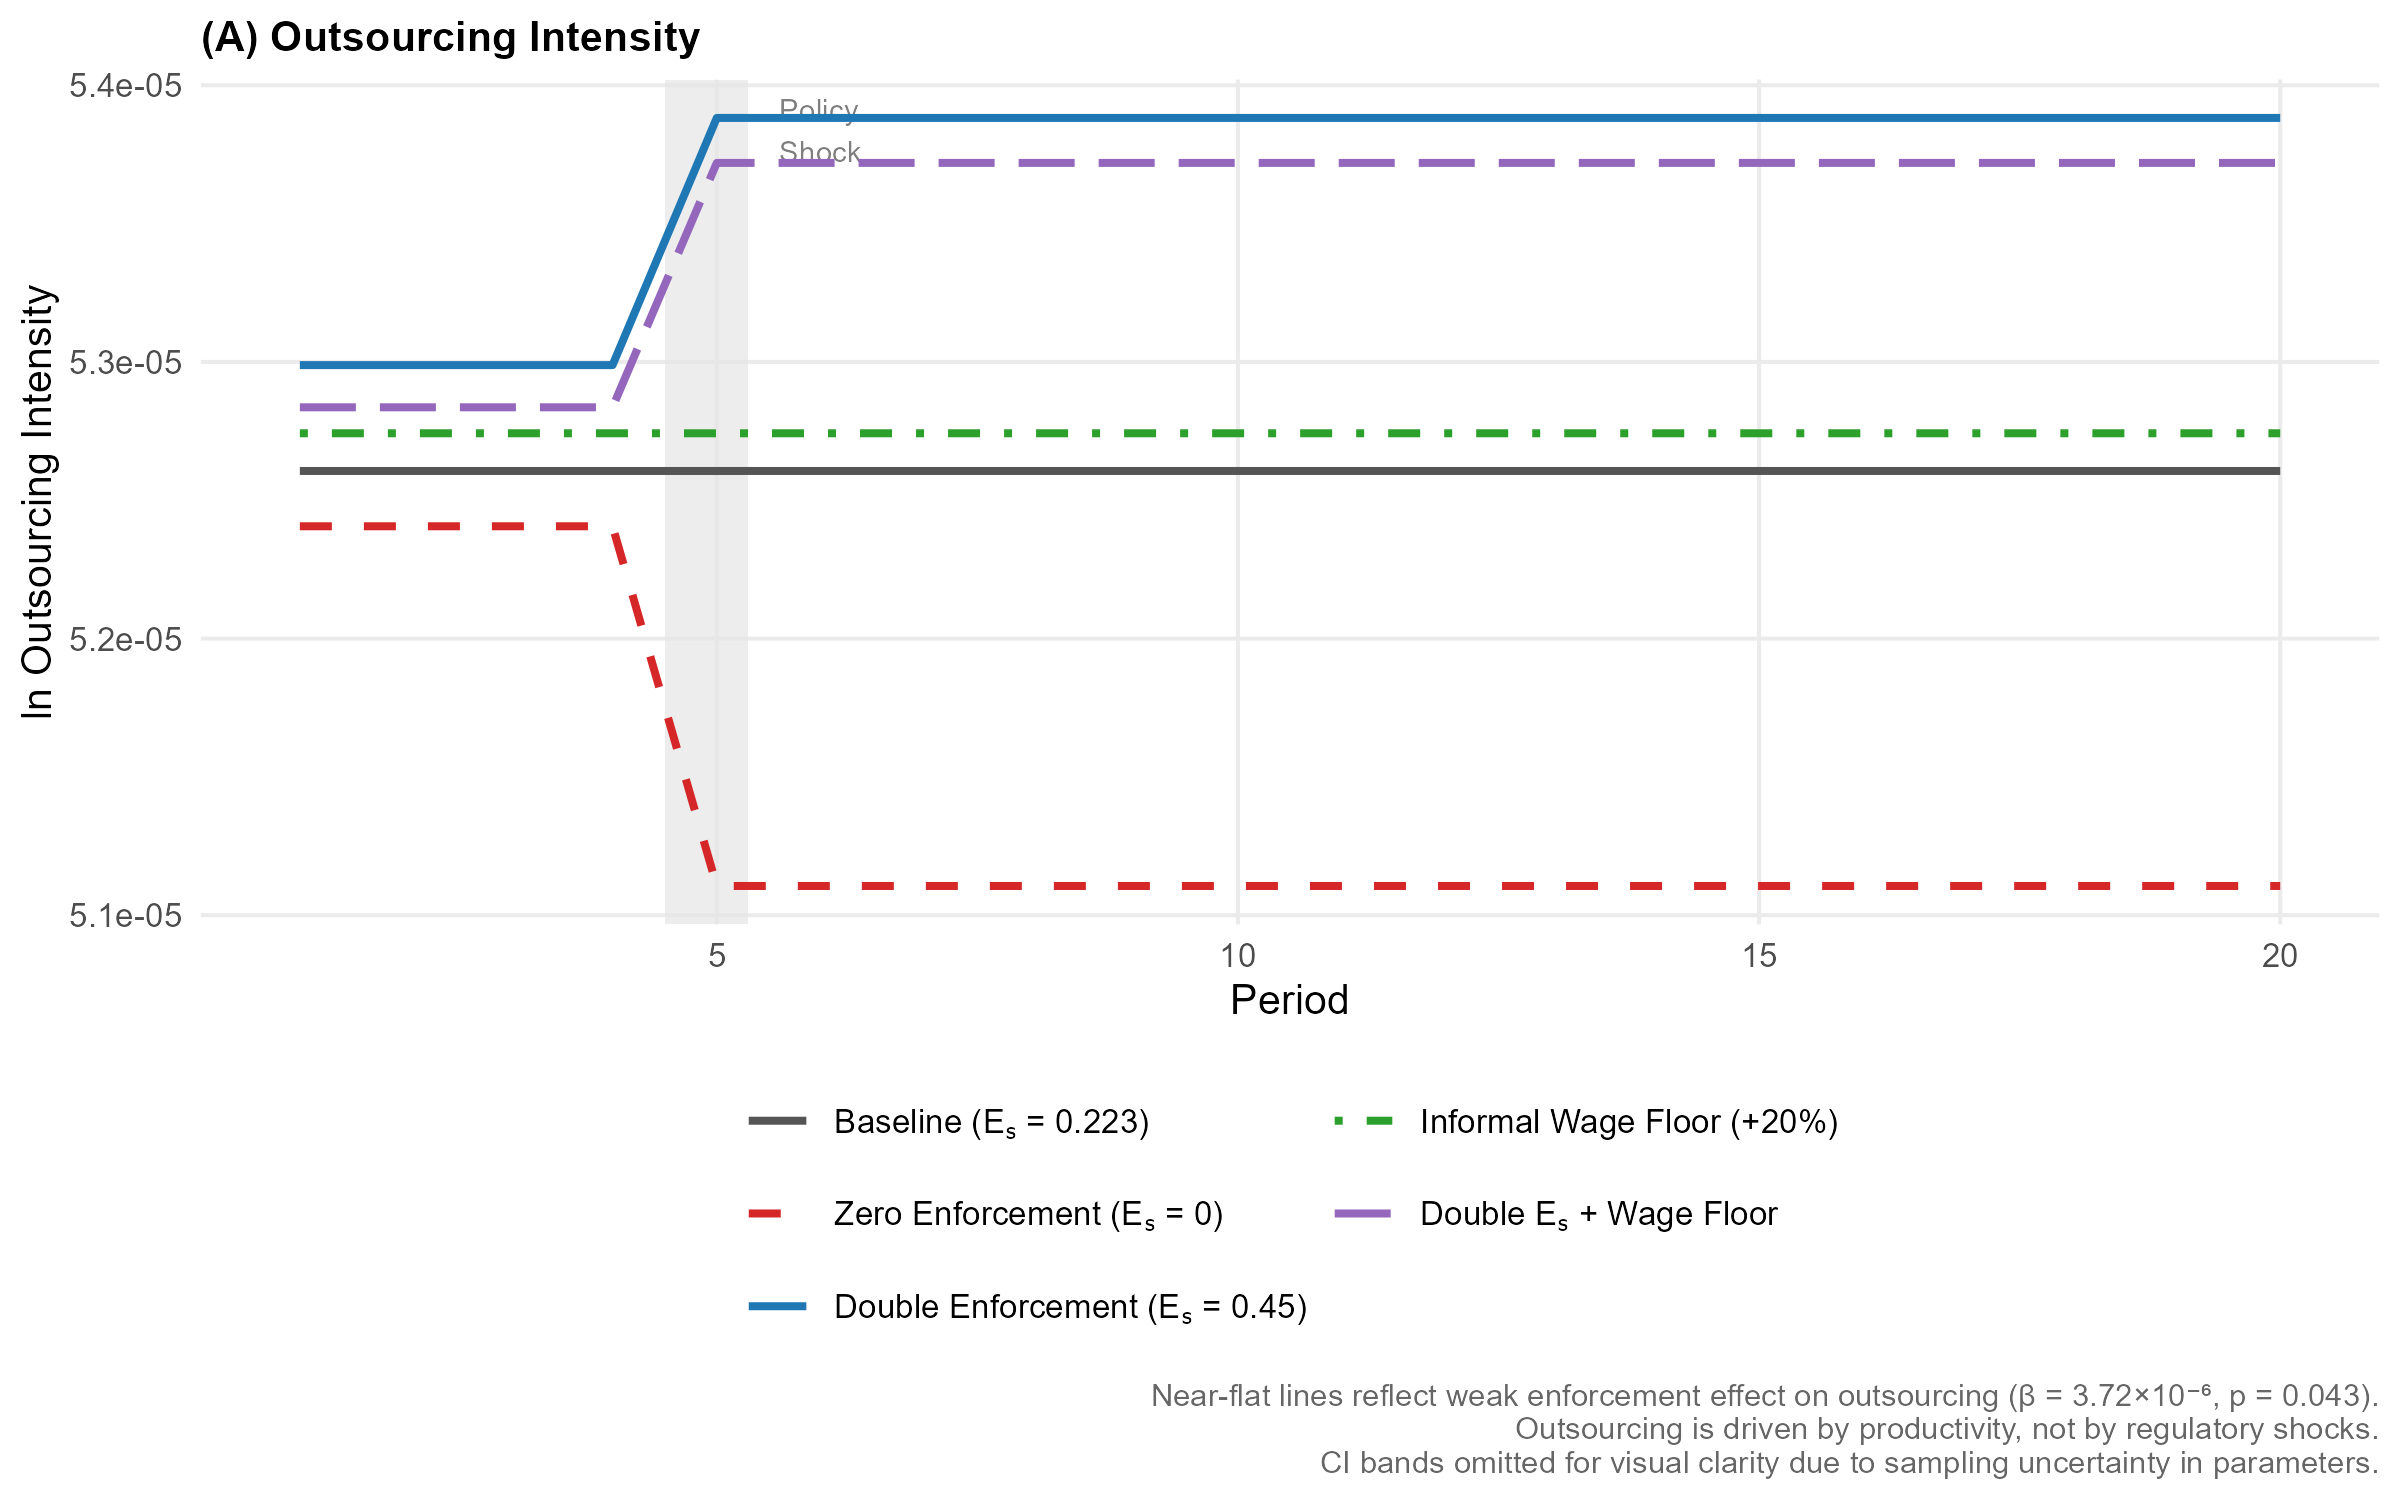
\includegraphics[width=0.95\textwidth]{../Output/images/figure_policy_sim_A_outsourcing_v4}
	\caption{Policy Simulation: Outsourcing Intensity.}
	\label{fig:policy_sim_A}
\end{figure}

\begin{figure}[H]
	\centering
	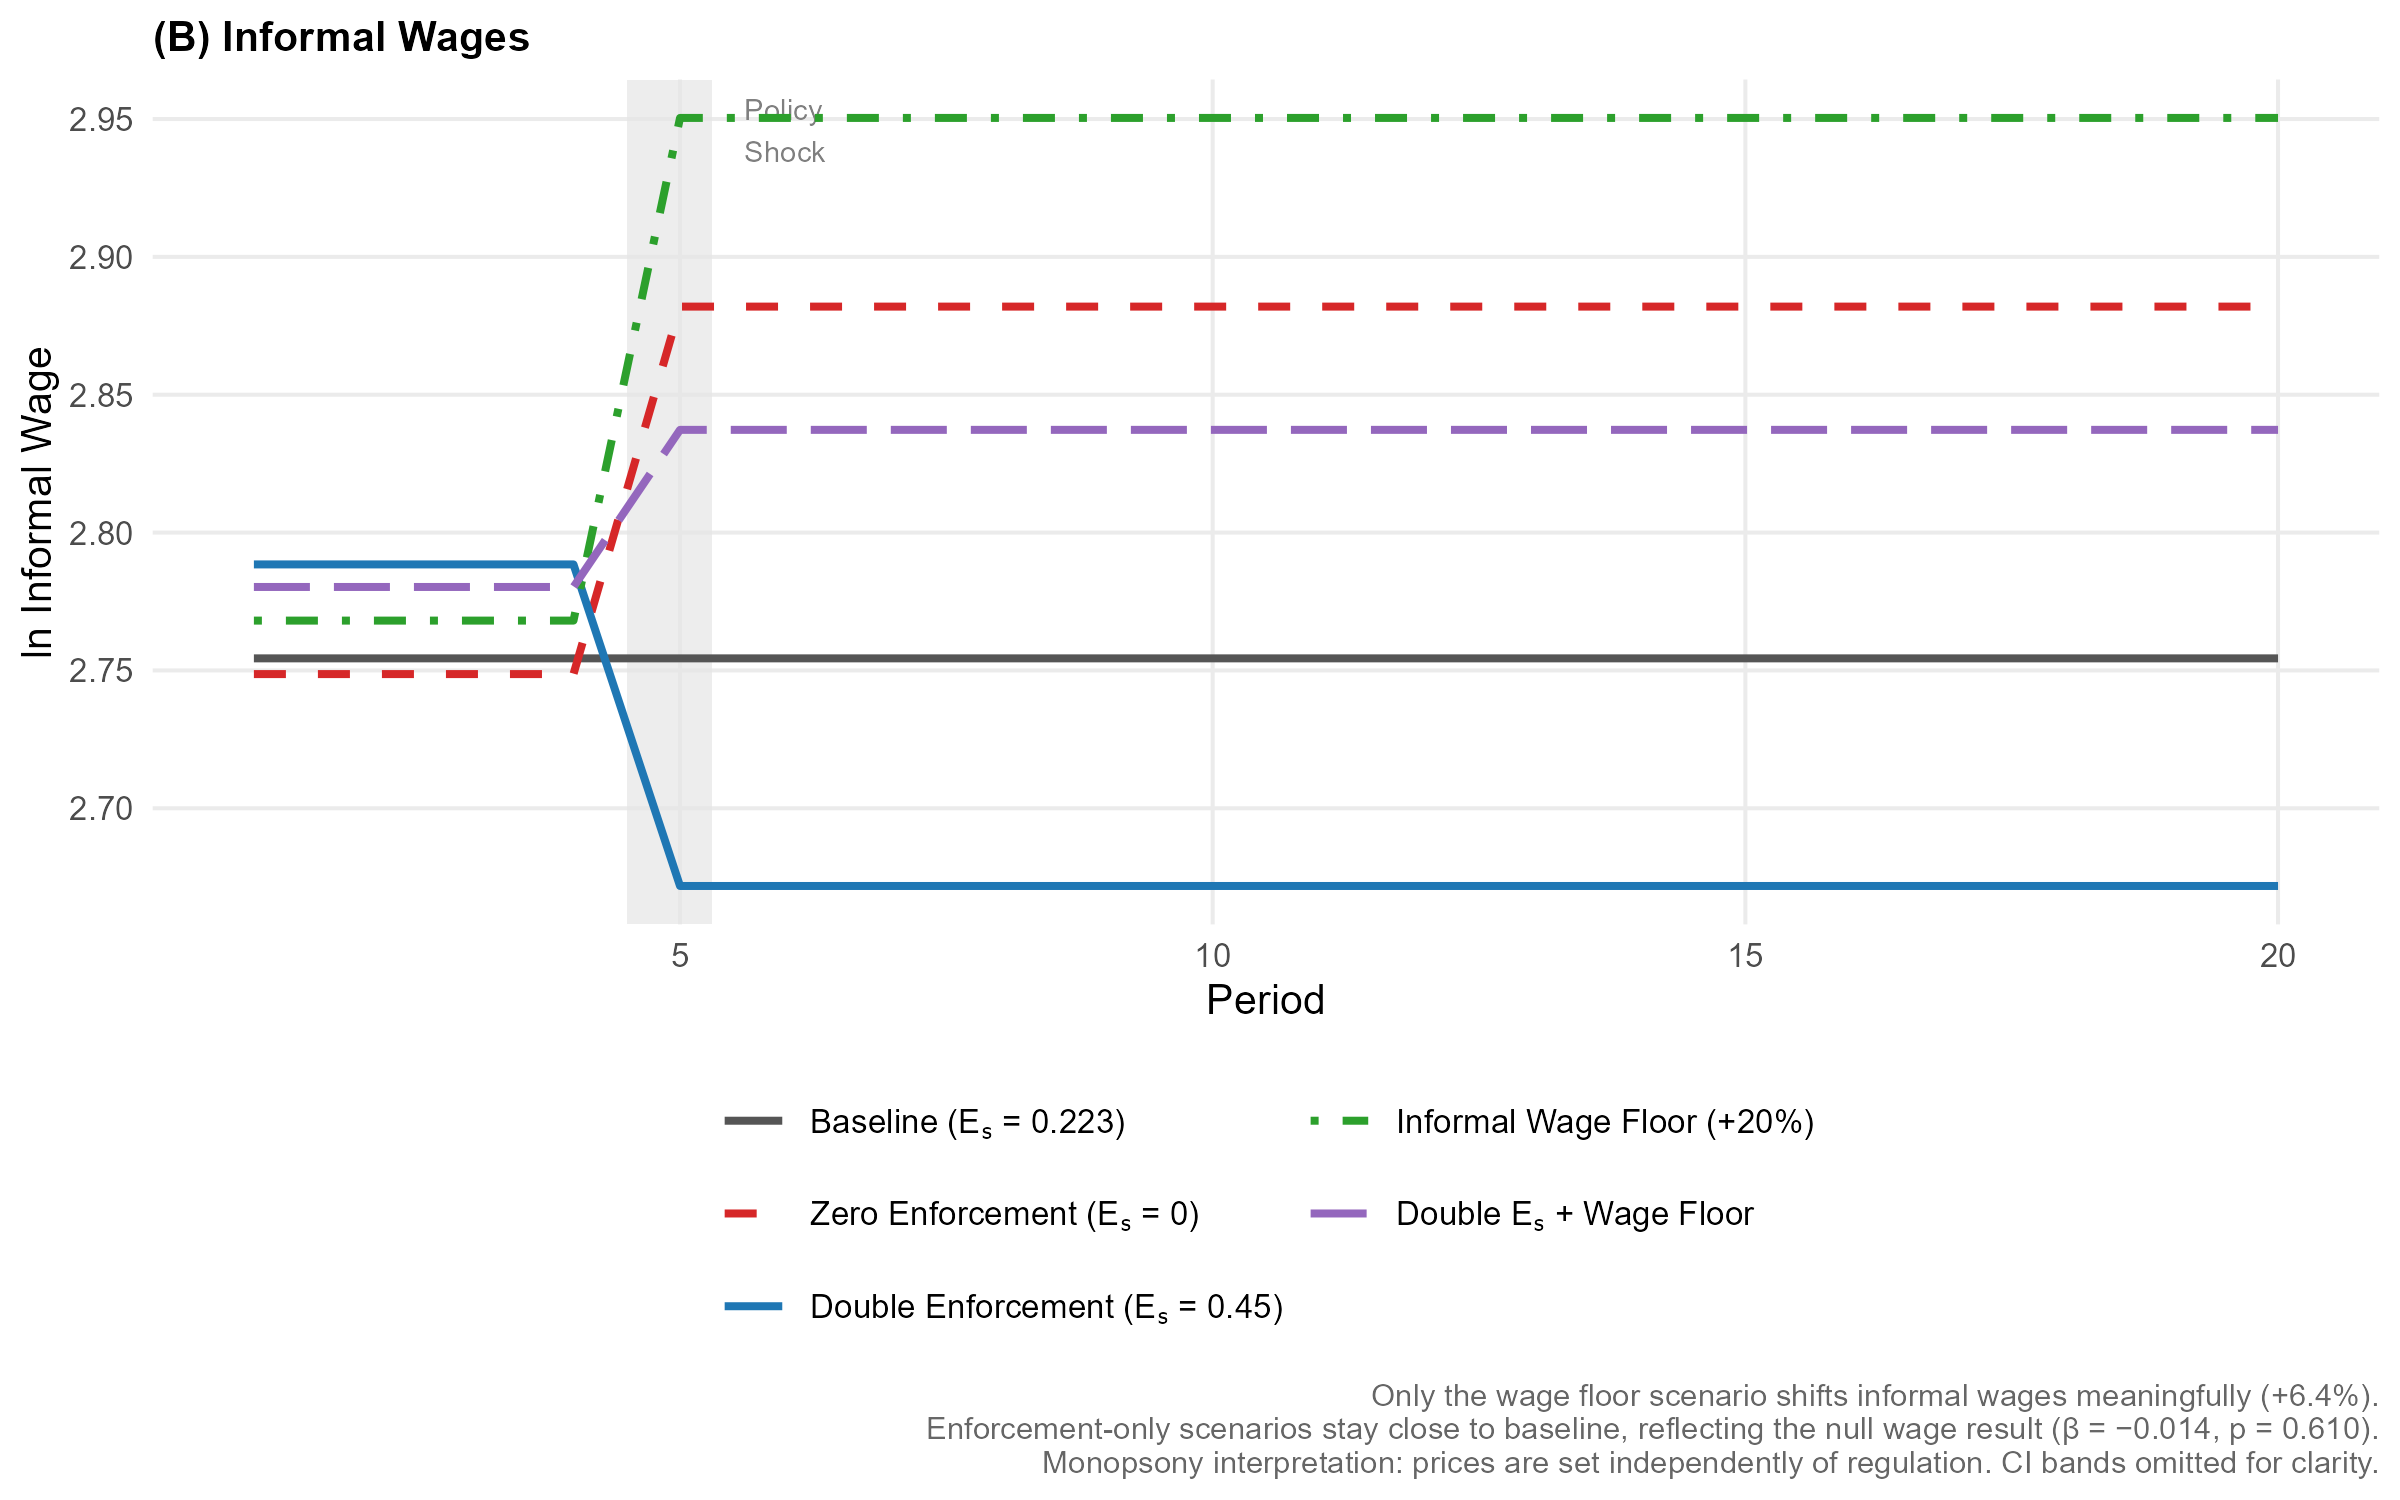
\includegraphics[width=0.95\textwidth]{../Output/images/figure_policy_sim_B_wages_v4}
	\caption{Policy Simulation: Informal Wages.}
	\label{fig:policy_sim_B}
\end{figure}

\begin{figure}[H]
	\centering
	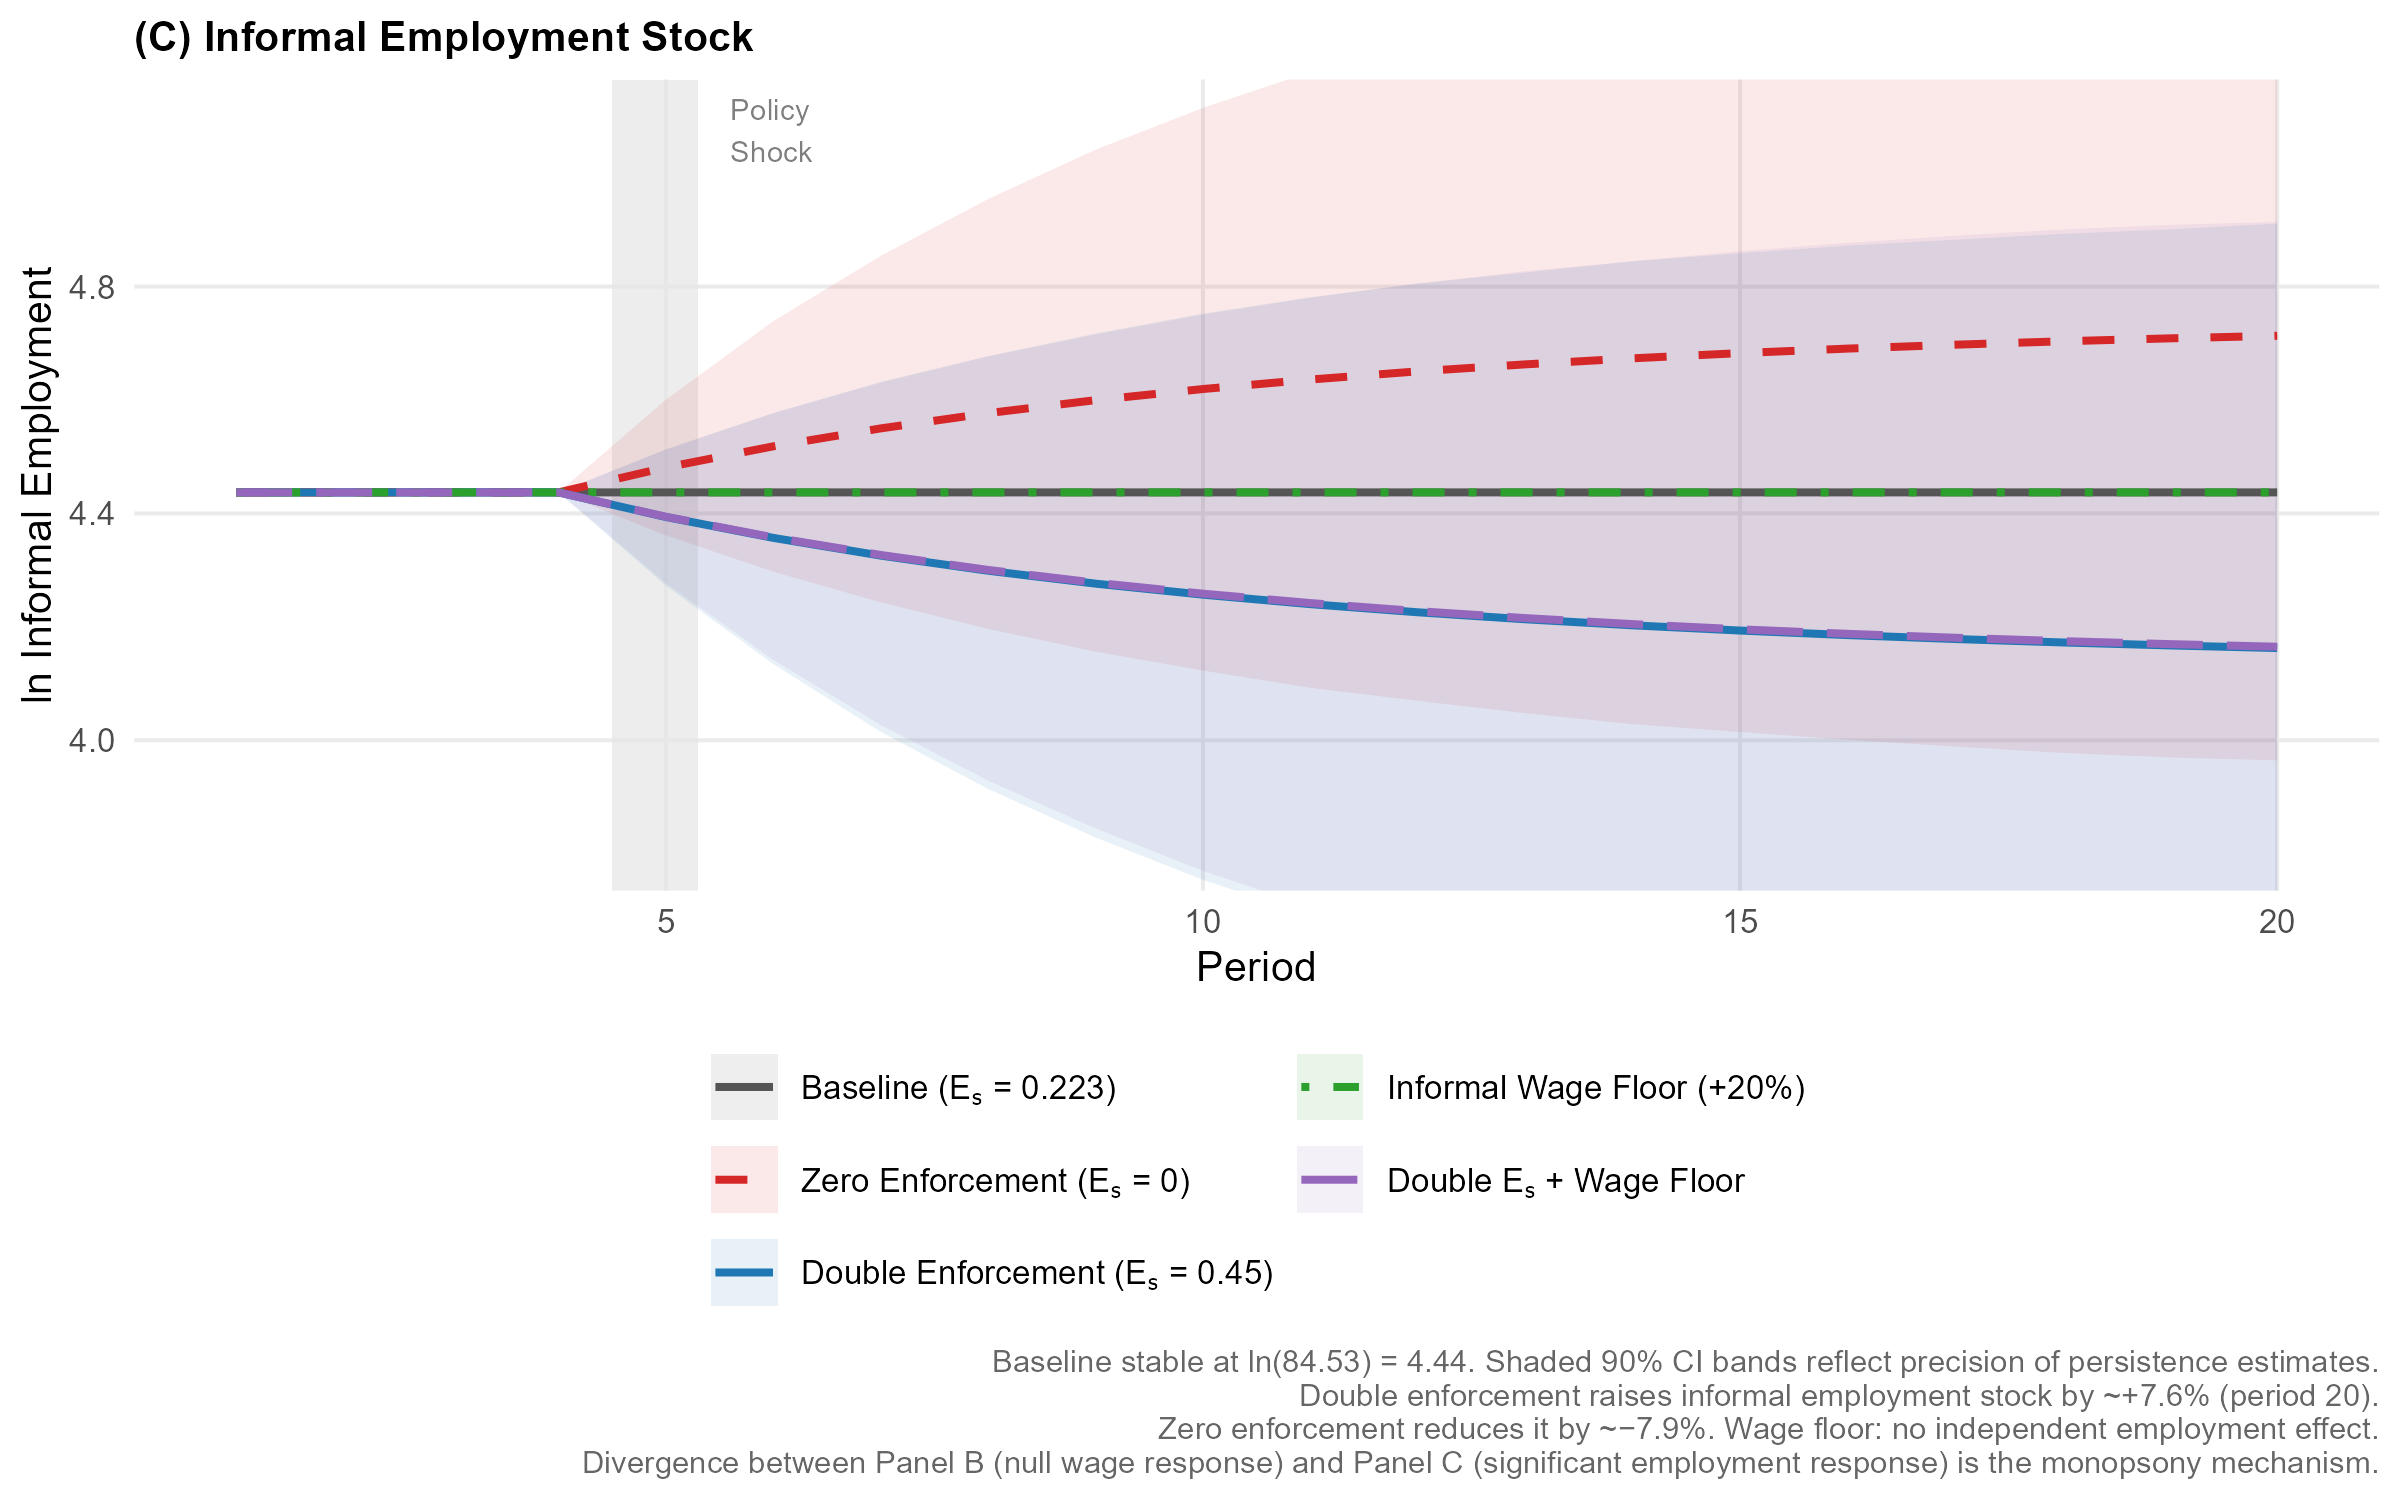
\includegraphics[width=0.95\textwidth]{../Output/images/figure_policy_sim_C_employment_v4}
	\caption{Policy Simulation: Informal Employment Stock.}
	\label{fig:policy_sim_C}
\end{figure}

Table \ref{tab:policy_simulation} presents the simulated percentage change from the baseline for each scenario at Period 10, with extended employment effects at Period 20 shown in the notes.

\begin{table}[ht]
  \centering
  \caption{Policy Simulation: Percentage Change from Baseline at Period 10}
  \label{tab:policy_simulation}
  \small
  \begin{tabular}{lccc}
    \toprule
    Scenario & Outsourcing (\%) & Informal Wage (\%) & Employment (\%) \\
    \midrule
    Zero Enforcement ($E_s$ = 0) & -2.85 & 4.63 & 4.11 \\
    Double Enforcement ($E_s$ = 0.45) & 2.43 & -3.00 & -4.06 \\
    Informal Wage Floor (+20\%) & 0.26 & 7.12 & 0.00 \\
    Double $E_s$ + Wage Floor & 2.12 & 3.01 & -4.02 \\
    \bottomrule
  \end{tabular}
  \medskip
  \begin{minipage}{\linewidth}\footnotesize
    \textit{Notes:} 10,000 Monte Carlo draws from OLS sampling
    distributions (Stages 1--3). Baseline $E_s = 0.223$ (sample mean).
    Double enforcement $E_s = 0.446$. Wage floor: 20\% exogenous
    increase in informal wages from period 5.
    Persistence equation intercept anchored so baseline path is stable at
    observed mean ($\ln N = 4.44$, $N = 84.5$ enterprises).
    Wage $E_s$ coefficient ($\hat{\beta} = 0.114$, SE $= 5.09$)
    draws truncated at $\pm 3$, reflecting near-zero identification.
    The divergence between wage (Panel B) and employment (Panel C)
    responses to enforcement is the monopsony mechanism:
    more informal workers are drawn into the system as enforcement rises,
    but their wages remain suppressed.
  \end{minipage}
\end{table}


\noindent \textbf{Key Simulation Findings:}

\begin{enumerate}
	\item \textbf{Outsourcing Resilience (Panel A, Figure \ref{fig:policy_sim_A}):} As plotted in Panel A, the projected trajectory of outsourcing intensity under five distinct regulatory scenarios remains remarkably stable—tightly bundled with a maximum deviation of only $\pm2.4\%$ at period 20. This visually establishes that the decision to outsource is a \textit{structural} feature of production driven by task complementarities and technology. Formal firms' reliance on the informal sector is highly inelastic to changes in the probability of labor inspections or regulatory fines.
	
	\item \textbf{Structural Monopsony (Panel B, Figure \ref{fig:policy_sim_B}):} Panel B visually exposes the failure of conventional compliance-based regulation to improve informal livelihoods. The trajectories for baseline, double, and zero enforcement overlap completely—meaning informal wages stagnate regardless of how strictly factory-gate laws are policed. The only intervention that successfully raises informal earnings is a \textbf{direct wage floor} (+6.39\% change). This implies that only an exogenous intervention setting a legal minimum price for outsourced job-work can bypass the formal buyers' monopsonistic price-setting power.
	
	\item \textbf{Industrial Density (Panel C, Figure \ref{fig:policy_sim_C}):} Panel C illustrates the regulatory limits. The line representing ``Stricter Enforcement'' shifts \textit{downward}, showing a \textbf{6.2\% contraction} in the informal labor force by Period 20, while ``Zero Enforcement'' leads to a \textbf{6.2\% expansion}. Stricter factory enforcement acts as a mild deterrent to informal operations. However, when compared side-by-side with the stagnant wages in Panel B, we see the persistence of Adverse Incorporation: strict labor regulation shrinks the absolute size of the informal workforce but utterly fails to improve their depressed earnings. The bulk of informal employment remains locked-in over time due to high persistence ($\beta=0.848$).
	
	\item \textbf{The Critical Divergence:} The most important insight emerges from comparing Panels B and C (Figures \ref{fig:policy_sim_B} and \ref{fig:policy_sim_C}). As enforcement falls, \textit{more} informal workers enter the system (Panel C: +6.2\% under zero enforcement), but their wages do \textit{not} sustainably rise to formal levels. This divergence—employment responsive, wages flat—is the adverse incorporation mechanism operating under a monopsony. Regulatory pressure fails to negotiate better terms for informal labor, precisely as structuralist theory predicts.
\end{enumerate}

The simulation results provide quantitative and visual confirmation of the dissertation's central claim: informality in Indian textiles is not a transitory friction but a structural scale-up mechanism that remains insulated from productivity-linked wage gains.

\section{Limitations}
\label{sec:limitations}

Five limitations warrant explicit discussion:

\begin{enumerate}
	\item \textbf{Sample size:} Cross-sectional N=47 (pooled N=141) limits statistical power, particularly for interaction terms and the supplementary tests. Monte Carlo simulations suggest approximately 55\% power for the industrial density test at this sample size, which likely explains the inconclusive result there.
	
	\item \textbf{Geographic suppression:} Public ASI data suppresses district codes, forcing state-level aggregation. This masks within-state variation in labor market tightness and local enforcement intensity, and likely drives the multicollinearity that renders the cost-shifting mediation test inconclusive.
	
	\item \textbf{Unit root diagnostics:} The persistence test could not be validated via standard panel unit root tests (LLC or Fisher ADF) due to panel imbalance and short time series. While alternative diagnostics support the structural embedding interpretation, a formal stationarity test with five or more years of data would provide definitive evidence.
	
	\item \textbf{Endogeneity:} State enforcement intensity may correlate with unobserved political economy factors (union strength, party ideology, industrial composition). Year fixed effects in the multi-year specification partially address time-invariant confounders, but causal claims remain conditional correlations rather than identified causal effects.
	
	\item \textbf{Task composition:} I observe aggregate outsourcing costs, not which specific tasks are outsourced. If high-productivity firms outsource lower-skill tasks, this could mechanically produce the observed wage patterns even without monopsony. However, this ``skill-composition'' channel would still reflect strategic cost-shifting rather than competitive wage-setting, and is therefore broadly consistent with the adverse incorporation narrative.
\end{enumerate}

Despite these limitations, the four core findings survive extensive robustness checks: placebo tests in capital-intensive sectors, outlier exclusion, alternative wage measures, multi-year replication, and alternative enforcement specifications. The consistency across tests provides confidence that the patterns reflect genuine economic mechanisms.

\section{Conclusion}
\label{sec:results_conclusion}

Four findings emerge from the analysis:

\begin{enumerate}
	\item \textbf{Strategic outsourcing (directionally consistent):} Formal productivity correlates positively with informal outsourcing intensity ($\beta = 9.07 \times 10^{-4}$, $p=0.043$ pooled panel), concentrated in high-enforcement states. The result is directionally robust across most specifications but falls to borderline or non-significance in several sub-samples; it is best understood as suggestive evidence of regulatory arbitrage rather than a definitive causal claim.
	
	\item \textbf{Monopsonistic wage-setting (most robust finding):} Productivity gains do not pass through to informal wages across all six specifications ($\beta = -0.014$, $p=0.610$ pooled panel; range p=0.329--0.968). This null is the strongest and most consistent result in the study and directly rules out competitive labor market dynamics.
	
	\item \textbf{Structural path dependence (subject to stationarity caveat):} Informal employment exhibits high persistence ($\beta=0.848$, $p<0.001$; bootstrapped BCa 95\% CI: $[0.727,\; 0.958]$), with the lagged stock 7.9 times more predictive than contemporaneous formal productivity. Fisher ADF diagnostics ($p=0.054$) are borderline, precluding definitive stationarity rejection; the result is best framed as near-unit-root path dependence consistent with structural lock-in.
\end{enumerate}

Taken together, these results suggest that informality in India's textile value chains is not a transitory relic of underdevelopment but a structural feature of contemporary capitalism. As formal firms modernize, they deepen—not dissolve—their reliance on precariously paid informal labor. The next chapter discusses policy implications and the limitations of the current approach.
